\documentclass[10pt]{article}

\usepackage[a4paper,margin=20mm]{geometry}
\usepackage[T1]{fontenc}
\usepackage[utf8]{inputenc}
\usepackage{amsmath,amssymb}
\usepackage{array,booktabs}
\usepackage{longtable}
\usepackage{graphicx}
\usepackage{float}
\usepackage{xcolor}
\usepackage{tikz}
\usetikzlibrary{arrows.meta,positioning,shapes.geometric,fit,backgrounds,calc}
\usepackage[numbers,sort&compress]{natbib}
\usepackage[colorlinks=true,linkcolor=blue!55!black,citecolor=blue!55!black,urlcolor=blue!55!black]{hyperref}
\usepackage{url}

\graphicspath{{figures/}}
\setlength{\parindent}{0pt}
\setlength{\parskip}{5pt}
\setlength{\tabcolsep}{4.5pt}
\renewcommand{\arraystretch}{1.12}

\definecolor{fifo}{HTML}{4C78A8}
\definecolor{reservoir}{HTML}{F58518}
\definecolor{irgreen}{HTML}{54A24B}
\definecolor{danger}{HTML}{E45756}
\definecolor{lightblue}{HTML}{DBE9F6}
\definecolor{lightorange}{HTML}{FCE5CC}
\definecolor{lightgreen}{HTML}{DCEFD9}

\newcommand{\fifo}{\textsc{FIFO}}
\newcommand{\res}{\textsc{Reservoir}}
\newcommand{\ir}{\textsc{IR}}
\newcommand{\pct}[1]{#1\%}
\newcommand{\pp}{\,pp}

\title{\textbf{From Reservoir Replay to Critic-Free Imagined Rehearsal\\in Sequential RLScape}\\[3pt]
\large A chronological experimental chapter on retention, model semantics,\\critic failure, and controlled actor recovery}
\author{Steven Davenport\\Continual Reinforcement Learning Research Notes}
\date{Experiments completed August 2026; expanded report generated 13 August 2026}

\begin{document}
\maketitle

\begin{abstract}
This chapter records a chronological sequence of three linked studies in a goal-conditioned DreamerV3 agent operating in RLScape. Study I compares a 200k-capacity global FIFO replay against a persistent, goal-stratified episode reservoir while one agent learns \emph{kill goblin}, \emph{bury bones}, and \emph{chop logs} for 500k environment steps each. Reservoir replay produced strong but transient balanced retention: at 1.25M steps its worst sampled-policy goal reached \pct{49} versus \pct{8} for FIFO, but by 1.5M all reservoir goals had collapsed to at most \pct{16}. Ungated actor-only imagined rehearsal (IR) was likewise conditional and often harmful. Study II audits the strong 1.25M and collapsed 1.5M checkpoints on an identical replay-state bank. Reward and continuation heads accurately recognize factual completion events but barely respond to the requested one-hot goal; the critic is severely overoptimistic and becomes more optimistic as real behavior deteriorates. An exact six-step imagination audit then shows that \pct{94.4}--\pct{97.3} of the IR lambda-return target comes from critic bootstrap, while entropy contributes only about \pct{1}--\pct{2} of the measured actor-loss magnitude. Study III converts these diagnoses into a controlled recovery assay: only the actor is zero-mask corrupted, all other parameters are frozen, and 15 recovery conditions are evaluated in 6,750 paired real-environment episodes. Standard and entropy-off IR remain weak or destructive. Removing critic bootstrap changes the result decisively: reward-only IR reaches \pct{73.0} mean sampled success at $H=15$ and \pct{85.3} mean deterministic success at $H=20$, compared with \pct{28.3} and \pct{41.3} for the corrupted actor and \pct{56.3} and \pct{49.3} for the clean actor. The combined evidence establishes that imagined actor adaptation is viable in this domain, but its current critic bootstrap is the primary harmful teaching signal. Counterfactual goal training, conservative value use, and prespecified adaptation gates remain the next requirements for a continual-learning algorithm rather than a controlled recovery mechanism.
\end{abstract}

\tableofcontents
\clearpage

\section{Research programme and chronological evidence chain}

The long-term research direction is continual reinforcement learning over an RLScape task landscape: train on goals $A\rightarrow B\rightarrow C\rightarrow\cdots$, repeatedly evaluate all previous goals, and measure both forgetting and transfer speed relative to a non-IR baseline. The immediate question was narrower. The preceding FIFO experiment suggested that later phases remove most early-task data, potentially weakening the goal-conditioned reward model and value function that IR relies on. We therefore asked:

\begin{enumerate}
  \item Does goal-stratified reservoir replay preserve earlier goal competence better than global FIFO replay?
  \item Does a retained multi-goal world model and critic make actor-only IR useful at evaluation time?
  \item Can the system train continuously for 1.5M steps with research-grade checkpoint and evaluation integrity?
\end{enumerate}

The first experiment contributes a fully persisted three-goal sequential run, six immutable training checkpoints, 24 paired frozen/IR evaluation units, two action-selection modes, and a direct comparison to the previous FIFO run. It is an exploratory, single-seed systems experiment rather than a population-level statistical claim. The later experiments deliberately reuse the same pinned checkpoints. This converts a costly multi-day training run into a sequence of increasingly controlled mechanism tests.

The chapter is organized as a research diary without sacrificing paper-style separation between method, result, and interpretation:
\begin{enumerate}
  \item \textbf{Study I --- continual training and replay.} Establish whether reservoir replay preserves usable cross-goal knowledge and whether ordinary actor-only IR helps at checkpoints.
  \item \textbf{Study II --- subsystem and imagination audits.} Hold the replay-state bank fixed and locate whether failure lies in factual event recognition, counterfactual goal semantics, continuation, critic calibration, or the exact IR objective.
  \item \textbf{Study III --- controlled actor corruption and recovery.} Hold the world model and critics fixed, damage only the actor, and causally ablate horizon, entropy, and critic bootstrap.
\end{enumerate}

To keep implementation artifacts and thesis terminology aligned, the
canonical repository stages map to the paper studies as follows. Historical
run names beginning with \texttt{m} denote engineering milestones and are
retained only for provenance.

\begin{table}[H]
\centering
\caption{Canonical experiment identifiers used by the repository registry.}
\label{tab:canonicalstages}
\begin{tabular}{lll}
\toprule
Canonical ID & Experiment & Chapter location \\
\midrule
Stage 0 & Sequential reservoir baseline and checkpoint IR & Study I \\
Stage 1A & Same-state goal-conditioned head audit & Study IIa \\
Stage 1B & Exact imagination-path audit & Study IIb \\
Stage 2 & Controlled actor corruption and recovery & Study III \\
Stage 3A & Critic provenance and calibration audit & Planned \\
Stage 3B & Natural forgetting recovery & Planned \\
\bottomrule
\end{tabular}
\end{table}

\begin{figure}[H]
\centering
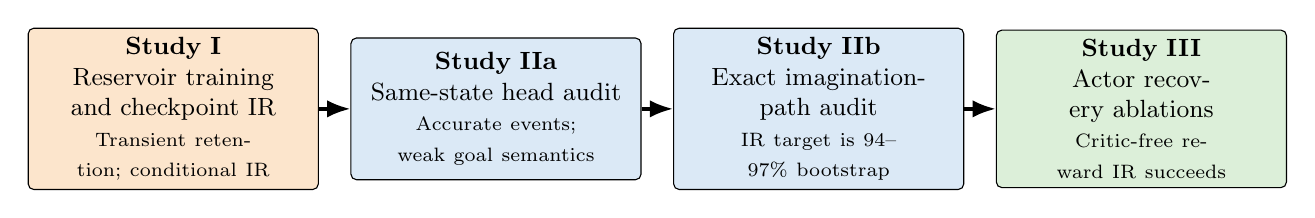
\begin{tikzpicture}[
  >=Latex,node distance=4mm,font=\small,
  bx/.style={draw,rounded corners=2pt,minimum height=18mm,text width=3.45cm,align=center},
  ar/.style={->,very thick}
]
\node[bx,fill=lightorange] (s1) {\textbf{Study I}\\Reservoir training and checkpoint IR\\\scriptsize Transient retention; conditional IR};
\node[bx,fill=lightblue,right=of s1] (s2) {\textbf{Study IIa}\\Same-state head audit\\\scriptsize Accurate events; weak goal semantics};
\node[bx,fill=lightblue,right=of s2] (s3) {\textbf{Study IIb}\\Exact imagination-path audit\\\scriptsize IR target is 94--97\% bootstrap};
\node[bx,fill=lightgreen,right=of s3] (s4) {\textbf{Study III}\\Actor recovery ablations\\\scriptsize Critic-free reward IR succeeds};
\draw[ar] (s1)--(s2);
\draw[ar] (s2)--(s3);
\draw[ar] (s3)--(s4);
\end{tikzpicture}
\caption{Chronological experimental logic. Each study was designed after observing the previous result; later tests reuse the same immutable checkpoints and therefore isolate mechanisms without another continual-training run.}
\label{fig:evidencechain}
\end{figure}

\section{Study I: sequential reservoir replay and checkpoint IR}

\subsection{Task sequence}

The agent trained on three goals in a fixed curriculum:

\begin{figure}[H]
\centering
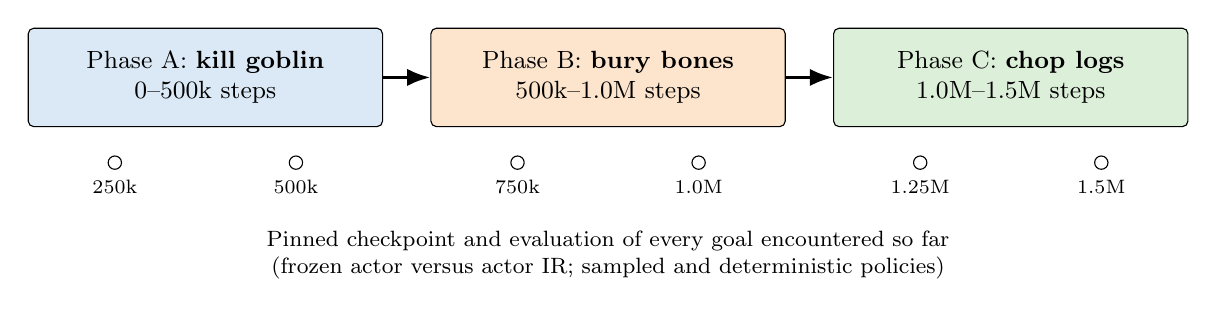
\begin{tikzpicture}[
  >=Latex,
  phase/.style={draw,rounded corners=2pt,minimum width=4.5cm,minimum height=1.25cm,align=center,font=\small},
  eval/.style={draw,circle,fill=white,inner sep=1.7pt,font=\scriptsize},
  arrow/.style={->,very thick}
]
\node[phase,fill=lightblue] (a) {Phase A: \textbf{kill goblin}\\0--500k steps};
\node[phase,fill=lightorange,right=6mm of a] (b) {Phase B: \textbf{bury bones}\\500k--1.0M steps};
\node[phase,fill=lightgreen,right=6mm of b] (c) {Phase C: \textbf{chop logs}\\1.0M--1.5M steps};
\draw[arrow] (a) -- (b);
\draw[arrow] (b) -- (c);
\foreach \x/\lab in {-1.15/250k,1.15/500k} {\node[eval] at ($(a.south)+(\x,-.45)$) {}; \node[below,font=\scriptsize] at ($(a.south)+(\x,-.55)$) {\lab};}
\foreach \x/\lab in {-1.15/750k,1.15/1.0M} {\node[eval] at ($(b.south)+(\x,-.45)$) {}; \node[below,font=\scriptsize] at ($(b.south)+(\x,-.55)$) {\lab};}
\foreach \x/\lab in {-1.15/1.25M,1.15/1.5M} {\node[eval] at ($(c.south)+(\x,-.45)$) {}; \node[below,font=\scriptsize] at ($(c.south)+(\x,-.55)$) {\lab};}
\node[below=12mm of b,font=\footnotesize,align=center] {Pinned checkpoint and evaluation of every goal encountered so far\\(frozen actor versus actor IR; sampled and deterministic policies)};
\end{tikzpicture}
\caption{Sequential curriculum and evaluation ladder. There is no return phase in this experiment. The checkpoints permit later ablations without retraining the full curriculum.}
\label{fig:timeline}
\end{figure}

Each episode was capped at 200 actions and used sparse binary task-completion reward. The action interface was a flat $28\times18$ click grid, giving 504 discrete click locations. This was intentionally held fixed between replay conditions so the comparison isolates replay, not environment design.

\subsection{Agent and training configuration}

The implementation uses DreamerV3 \citep{hafner2023dreamerv3} with the repository's ``50m'' preset. The observed trainable parameter count was approximately 77.3M; the preset name is therefore a configuration label, not the measured parameter total. The recurrent state-space model (RSSM) uses a deterministic state of width 4,096 and a $32\times32$ categorical stochastic state. Training used batches of 8 sequences, sequence length 32, imagination horizon 15, training ratio 32, and bfloat16 computation on a 24,GB GPU.

Let $o_t$ be the image, $a_t$ the click action, and $s_t=(h_t,z_t)$ the Dreamer latent state. The goal-agnostic dynamics are
\begin{align}
 h_t &= f_\phi(h_{t-1},z_{t-1},a_{t-1}),\\
 z_t &\sim q_\phi(z_t\mid h_t,e_\phi(o_t)) \quad\text{during representation learning},\\
 z_t &\sim p_\phi(z_t\mid h_t) \quad\text{during imagination}.
\end{align}
Five RLScape goals are represented by a five-dimensional one-hot vector $g_t$, although only three goal IDs occur in this experiment. The behavior feature is
\begin{equation}
 x_t=[h_t;z_t;g_t].
\end{equation}
The reward, continuation, actor, value, and slow-value heads consume $x_t$:
\begin{align}
 \hat r_t&\sim p_\phi(r_t\mid h_t,z_t,g_t), &
 \hat c_t&\sim p_\phi(c_t\mid h_t,z_t,g_t),\\
 a_t&\sim\pi_\theta(a_t\mid h_t,z_t,g_t), &
 v_\psi&=v_\psi(h_t,z_t,g_t).
\end{align}
The RSSM transition and visual representation remain goal-agnostic. Thus the shared latent should model what is happening on screen, while the heads interpret that state under the requested goal.

\begin{figure}[H]
\centering
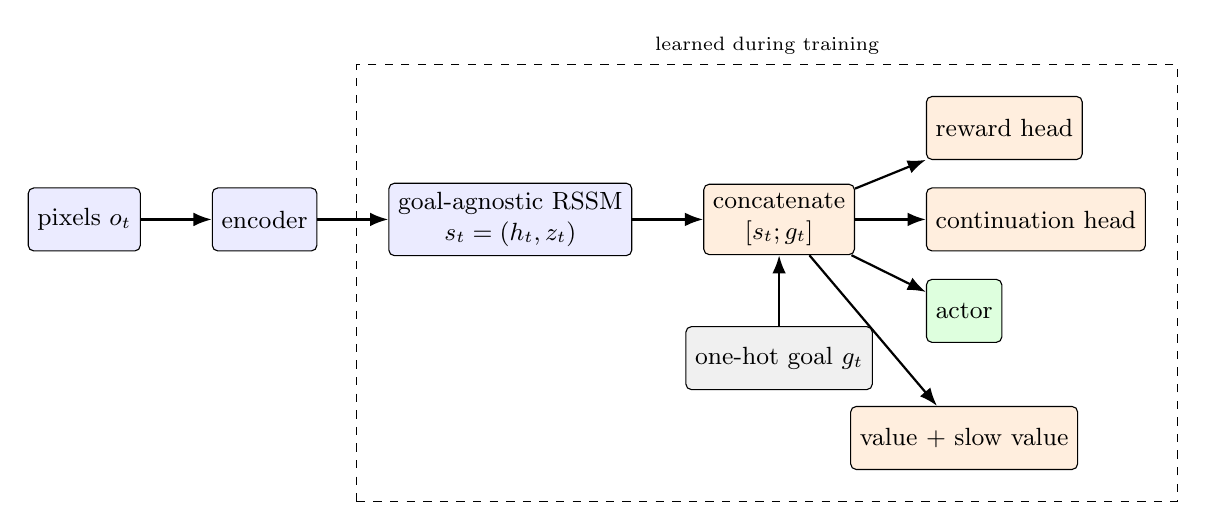
\begin{tikzpicture}[
  >=Latex,node distance=6mm and 9mm,
  box/.style={draw,rounded corners=2pt,minimum height=8mm,align=center,font=\small},
  frozen/.style={box,fill=blue!8},
  conditioned/.style={box,fill=orange!13},
  trainable/.style={box,fill=green!13},
  flow/.style={->,thick}
]
\node[frozen] (obs) {pixels $o_t$};
\node[frozen,right=of obs] (enc) {encoder};
\node[frozen,right=of enc] (rssm) {goal-agnostic RSSM\\$s_t=(h_t,z_t)$};
\node[conditioned,right=of rssm] (join) {concatenate\\$[s_t;g_t]$};
\node[conditioned,above right=3mm and 9mm of join] (rew) {reward head};
\node[conditioned,right=9mm of join] (cont) {continuation head};
\node[trainable,below right=3mm and 9mm of join] (actor) {actor};
\node[conditioned,below=8mm of actor] (value) {value + slow value};
\node[box,below=9mm of join,fill=gray!12] (goal) {one-hot goal $g_t$};
\draw[flow] (obs)--(enc); \draw[flow] (enc)--(rssm); \draw[flow] (rssm)--(join);
\draw[flow] (goal)--(join); \draw[flow] (join)--(rew); \draw[flow] (join)--(cont);
\draw[flow] (join)--(actor); \draw[flow] (join)--(value);
\node[draw,dashed,fit=(rssm)(join)(rew)(cont)(actor)(value),inner sep=4mm,label={[font=\scriptsize]above:learned during training}] {};
\end{tikzpicture}
\caption{Goal-conditioning architecture. During evaluation-time IR, only the actor parameters (green) are updated; the world model, reward/continuation heads, and critic/value functions are frozen.}
\label{fig:architecture}
\end{figure}

\subsection{Replay conditions}

\paragraph{FIFO baseline.}
The comparison run used the original global replay with capacity 200,000 sequence starts. Once full, newly collected experience evicts the oldest experience regardless of goal. Uniform training batches therefore increasingly reflect the current phase.

\paragraph{Goal-stratified episode reservoir.}
The new replay stores at most $M_g=1{,}000$ complete episodes independently for each represented goal, for a total capacity of 3,000 episodes. Within goal $g$, the $n_g$th observed episode is processed by Algorithm R \citep{vitter1985reservoir}:
\begin{equation}
 \Pr(\text{admit episode }n_g)=\min\left(1,\frac{M_g}{n_g}\right).
\end{equation}
If admitted after the group is full, it uniformly replaces one of the $M_g$ resident episodes. Consequently every historical episode for a goal has equal probability $M_g/n_g$ of residing in that goal's reservoir. Training samples a represented goal uniformly, an episode uniformly within that goal, and then a random sequence start. Short fragments are concatenated with explicit \texttt{is\_first} boundaries so the recurrent state resets correctly.

\begin{figure}[H]
\centering
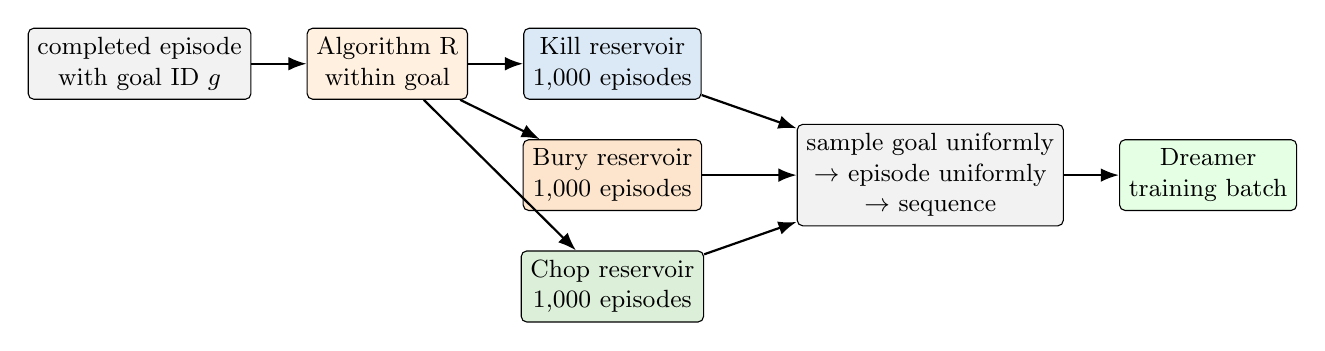
\begin{tikzpicture}[
  >=Latex,node distance=5mm and 7mm,font=\small,
  bx/.style={draw,rounded corners=2pt,minimum height=8mm,align=center},
  ar/.style={->,thick}
]
\node[bx,fill=gray!10] (stream) {completed episode\\with goal ID $g$};
\node[bx,fill=orange!12,right=of stream] (alg) {Algorithm R\\within goal};
\node[bx,fill=lightblue,right=of alg] (r1) {Kill reservoir\\1,000 episodes};
\node[bx,fill=lightorange,below=of r1] (r2) {Bury reservoir\\1,000 episodes};
\node[bx,fill=lightgreen,below=of r2] (r3) {Chop reservoir\\1,000 episodes};
\node[bx,fill=gray!10,right=12mm of r2] (sample) {sample goal uniformly\\$\rightarrow$ episode uniformly\\$\rightarrow$ sequence};
\node[bx,fill=green!10,right=of sample] (batch) {Dreamer\\training batch};
\draw[ar] (stream)--(alg);
\draw[ar] (alg)--(r1); \draw[ar] (alg)--(r2); \draw[ar] (alg)--(r3);
\draw[ar] (r1)--(sample); \draw[ar] (r2)--(sample); \draw[ar] (r3)--(sample);
\draw[ar] (sample)--(batch);
\end{tikzpicture}
\caption{Goal-stratified episode reservoir. Statistical retention is uniform over the episode stream within each goal; optimization sampling is balanced across represented goals.}
\label{fig:reservoir}
\end{figure}

This balance changes the effective emphasis on new data. The global training ratio remains 32, but the expected share of updates drawn from the current goal is 1, $1/2$, and $1/3$ in phases A, B, and C. In this limited sense, current-goal exposure is approximately 32, 16, and 10.7 replayed samples per environment step. This is a plausible source of slower acquisition or instability and is important when interpreting the comparison.

\subsection{Evaluation-time imagined rehearsal}

IR performs temporary test-time optimization of the actor from the agent's current latent state. For each environment action, Monte Carlo Posterior Batching (MCPB) draws $N=128$ posterior latent samples, imagines $H=6$ steps under the frozen world model, and takes one actor gradient update with learning rate $4\times10^{-5}$. MCPB is posterior batching: it does not denote particles and does not perform particle filtering, weighting, or resampling. The objective is the Dreamer actor objective: increase imagined, critic-estimated return while retaining the configured entropy bonus $\eta=3\times10^{-4}$,
\begin{equation}
 \theta' \leftarrow \theta-\alpha\nabla_\theta
 \left[-\mathbb E_{\hat\tau\sim p_\phi,\pi_\theta}
 \left(\widehat A_\psi(\hat\tau)+\eta\,\mathcal H[\pi_\theta(\cdot\mid \hat s,g)]\right)\right].
\end{equation}
The precise implementation uses the repository's normalized imagined-advantage actor loss. The world model, reward/continuation models, critic, and slow critic are frozen. Actor updates accumulate within an episode, are discarded at the episode boundary, and never alter the saved training checkpoint. There is no confidence, entropy, or value-based gate: IR runs at every action from the first action ($k=0$).

Conceptually, IR asks whether the retained model and critic contain enough goal-specific knowledge to repair a locally damaged actor without collecting gradient updates from the real reward stream. It is not hindsight relabeling \citep{andrychowicz2017her}: replay goals and rewards are not relabeled.

\subsection{Evaluation protocol and integrity}

At 250k-step intervals, every goal encountered by that point was evaluated. For each checkpoint--goal cell we ran:
\begin{itemize}
  \item 100 frozen and 100 IR episodes with sampled actions;
  \item 50 frozen and 50 IR episodes with deterministic actions.
\end{itemize}
Frozen and IR conditions used matching seed schedules and goal requests. Across 12 checkpoint--goal cells this yielded 3,600 episodes in 48 complete conditions (24 frozen/IR pairs). Requested episode counts, goal IDs, reset counts, return codes, and checkpoint parameter digests passed the evaluator's integrity checks. Because frozen and IR conditions ran in separate RLScape process lifetimes, their initial image hashes were not identical despite matching seed/goal identities. The analysis therefore treats them as seed-paired aggregate comparisons, not guaranteed pixel-identical counterfactual trajectories.

The FIFO evaluation predates a fix to the strict frame-hash pairing checker: its queue recorded failure even though individual condition summaries completed. We use the complete first attempts at checkpoints through 1.5M steps descriptively. This caveat does not affect the reservoir run's own completion status.

\section{Study I results}

\subsection{Execution and systems outcome}

The reservoir experiment completed all six training milestones and all 24 paired evaluation units without a training restart. Training took approximately 62.3 hours, evaluation 19.7 hours, and the full workflow approximately 82 hours. This satisfies the operational objective: a multi-day continual experiment can train, checkpoint, resume evaluation, and terminate cleanly.

At 1.5M steps the reservoir contained exactly 1,000 episodes per goal, 18,574 historical episodes had been considered for admission, and the retained episodes comprised 265,802 transitions. The latest sampling interval drew 655, 652, and 693 batches from kill, bury, and chop respectively, demonstrating near-uniform goal selection. Replay occupied 28.5,GiB of host memory and the full process 34.3,GiB, leaving 22.9,GiB available on the 62,GiB machine. Acting and training throughput were approximately 6.66 and 213 steps/s. The FIFO endpoint used 23.2,GiB for replay and 26.5,GiB for the process, with 6.92 acting steps/s and 222 training steps/s. The methods are therefore not memory-matched.

\begin{figure}[H]
\centering
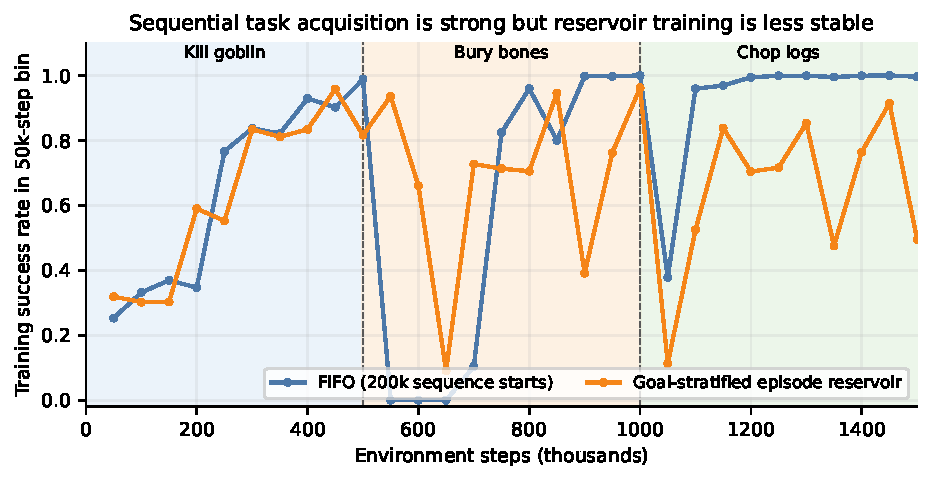
\includegraphics[width=.94\linewidth]{training_success.pdf}
\caption{Training success in successive 50k-step bins. FIFO learns each active task cleanly after an initial delay. Reservoir replay reaches high success on every phase but exhibits repeated large collapses, including late in the final phase. These are behavioral training metrics, not held-out evaluation.}
\label{fig:training}
\end{figure}

Reservoir training reached rolling 100-episode peaks of \pct{99}, \pct{100}, and \pct{100} on kill, bury, and chop, proving that the architecture and action interface can solve every chosen goal. Final rolling success was only \pct{85}, \pct{54}, and \pct{16}. In the last 10k steps of each phase, success was \pct{84.2}, \pct{37.5}, and \pct{11.3}. The main failure is therefore retention/stability, not basic reachability.

\begin{figure}[H]
\centering
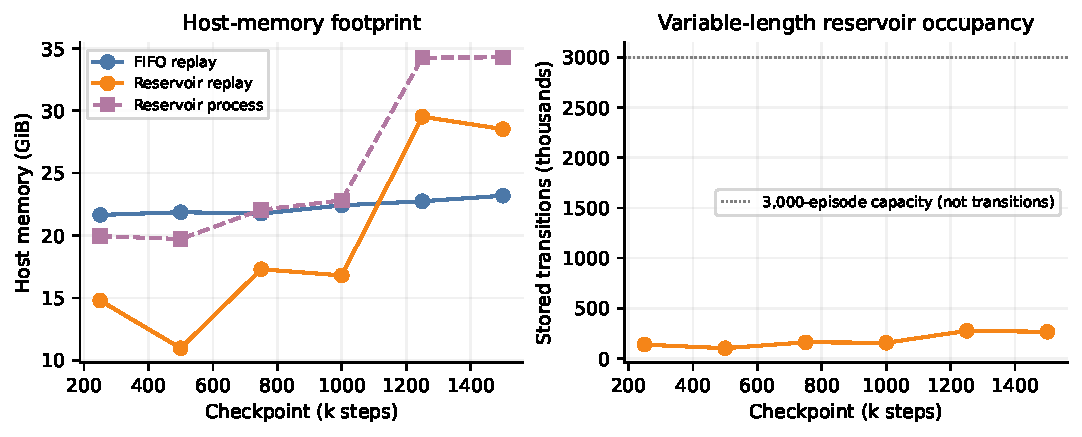
\includegraphics[width=.92\linewidth]{resource_footprint.pdf}
\caption{Resource use at pinned milestones. Episode capacity does not fix transition count because episode lengths vary. The 3,000-episode reservoir ended larger than the 200k-start FIFO buffer, making the comparison intentionally algorithmic rather than memory-matched.}
\label{fig:resources}
\end{figure}

\subsection{Frozen-policy checkpoint matrix}

\begin{figure}[H]
\centering
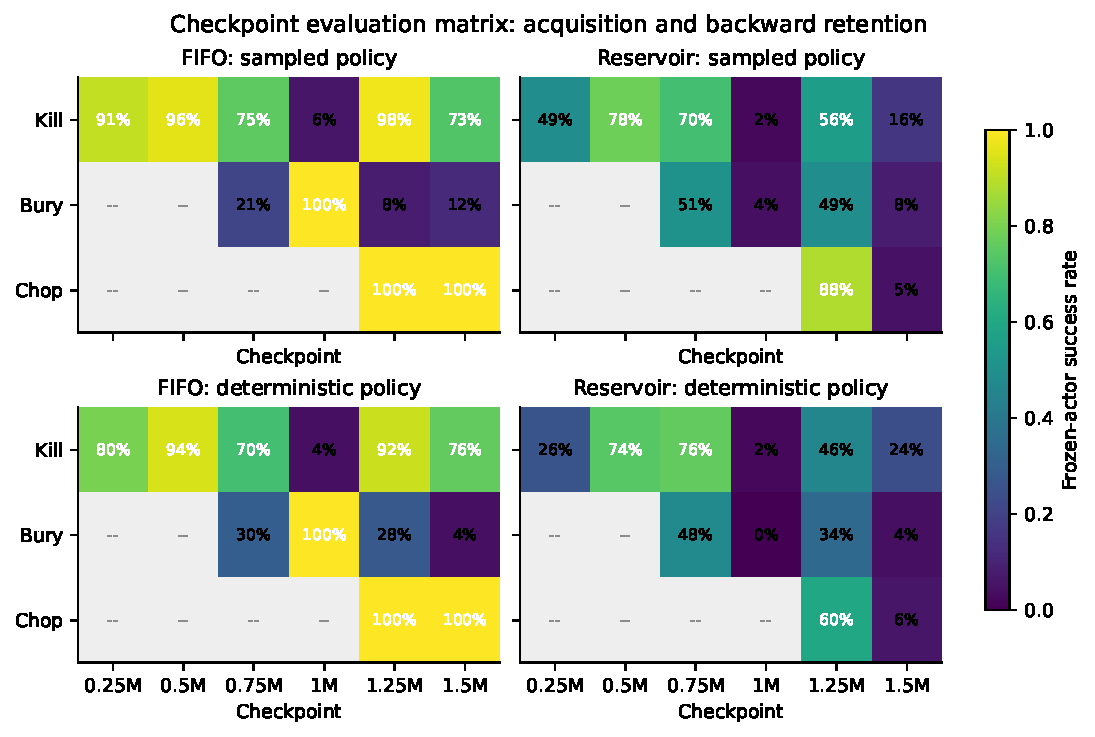
\includegraphics[width=.98\linewidth]{frozen_eval_heatmaps.pdf}
\caption{Frozen-actor success at all evaluable checkpoint--goal cells. Gray cells correspond to goals not yet introduced. The reservoir temporarily improves balanced retention but undergoes synchronized collapses at 1.0M and 1.5M steps.}
\label{fig:heatmaps}
\end{figure}

Across all available cells, FIFO frozen success averaged \pct{65.0} sampled and \pct{64.8} deterministic. Reservoir frozen success averaged \pct{39.7} and \pct{33.3}, a substantial overall deficit. On acquisition checkpoints---the end of the phase in which a goal was introduced---reservoir trailed FIFO by 38.8 points sampled and 48.3 points deterministic. Goal-balanced replay is therefore not a free retention improvement: it materially reduces or destabilizes current-task learning under the present update schedule.

The result is not uniformly negative. At 750k steps, after only 250k bury-bones training, reservoir sampled success was \pct{70} on kill and \pct{51} on bury; FIFO achieved \pct{75} and \pct{21}. The reservoir's worst task was therefore 30 points better. At 1.25M, after 250k chop training, reservoir simultaneously achieved \pct{56}, \pct{49}, and \pct{88}; FIFO achieved \pct{98}, \pct{8}, and \pct{100}. The reservoir's worst task was \pct{49} rather than \pct{8}. This is the clearest positive evidence: stored old-goal episodes, goal-balanced sampling, and goal-conditioned heads can jointly recover multiple skills while a new goal is being learned.

That balance was transient. At 1.0M, reservoir kill and bury collapsed to \pct{2} and \pct{4}; at 1.5M all three goals were \pct{16} or worse. FIFO showed selective forgetting instead: its final sampled scores were \pct{73}, \pct{12}, and \pct{100}. FIFO's retained mean was much higher, but its weakest old goal remained poor.

\begin{figure}[H]
\centering
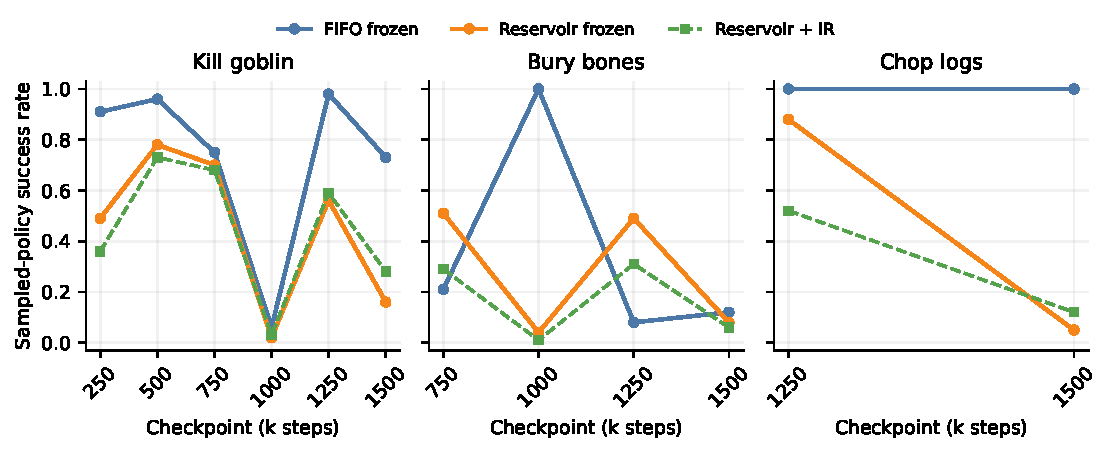
\includegraphics[width=.96\linewidth]{checkpoint_trajectories.pdf}
\caption{Sampled-policy trajectories for each goal. The dashed green line adds actor IR to the reservoir checkpoint. Reservoir skill recovery between 1.0M and 1.25M is followed by broad collapse between 1.25M and 1.5M.}
\label{fig:trajectories}
\end{figure}

\begin{figure}[H]
\centering
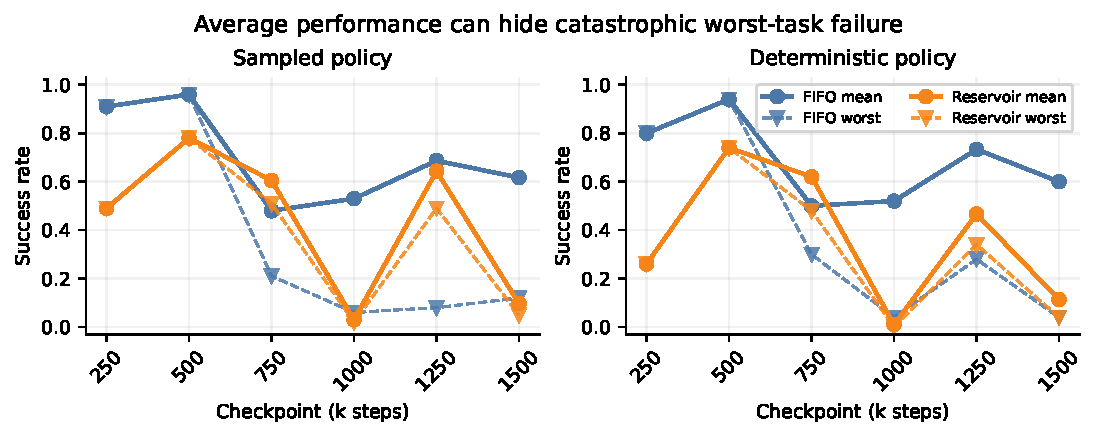
\includegraphics[width=.93\linewidth]{mean_and_worst_task.pdf}
\caption{Mean and worst encountered-goal performance. Reservoir replay has useful mid-phase worst-task advantages, while both methods can hide severe forgetting behind a reasonable mean.}
\label{fig:worst}
\end{figure}

\subsection{Forgetting}

Forgetting is reported as the maximum checkpoint success for a goal minus its final-checkpoint success. In the sampled reservoir evaluations it was 62 points for kill, 43 for bury, and 83 for chop. FIFO forgetting was 25, 88, and 0 points. Deterministic reservoir forgetting was 52, 44, and 54 points, versus 18, 96, and 0 for FIFO. Reservoir failure was broad; FIFO failure was concentrated in bury bones.

\begin{figure}[H]
\centering
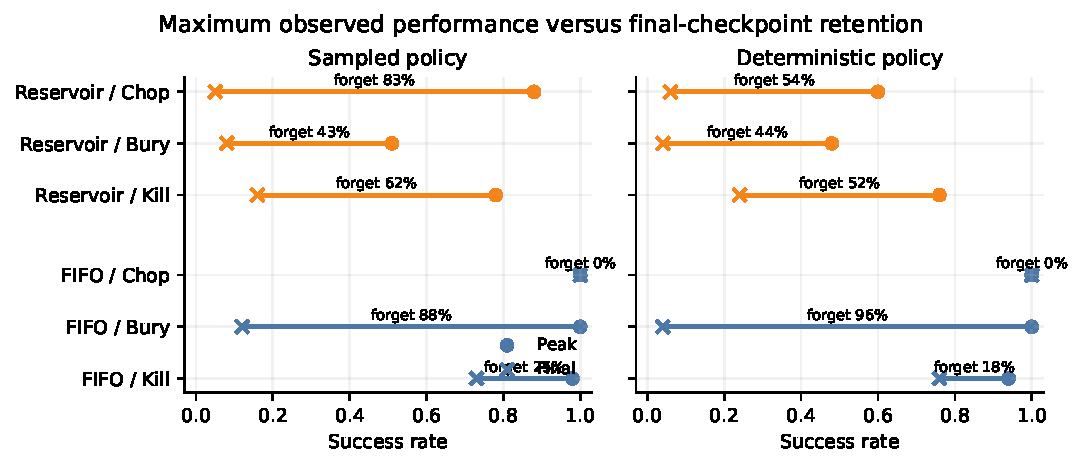
\includegraphics[width=.92\linewidth]{peak_to_final_forgetting.pdf}
\caption{Peak-to-final forgetting. Circles mark the best observed checkpoint and crosses mark the final checkpoint. A useful continual learner should keep both markers high and close together.}
\label{fig:forgetting}
\end{figure}

\subsection{Effect of iterative rehearsal}

\begin{figure}[H]
\centering
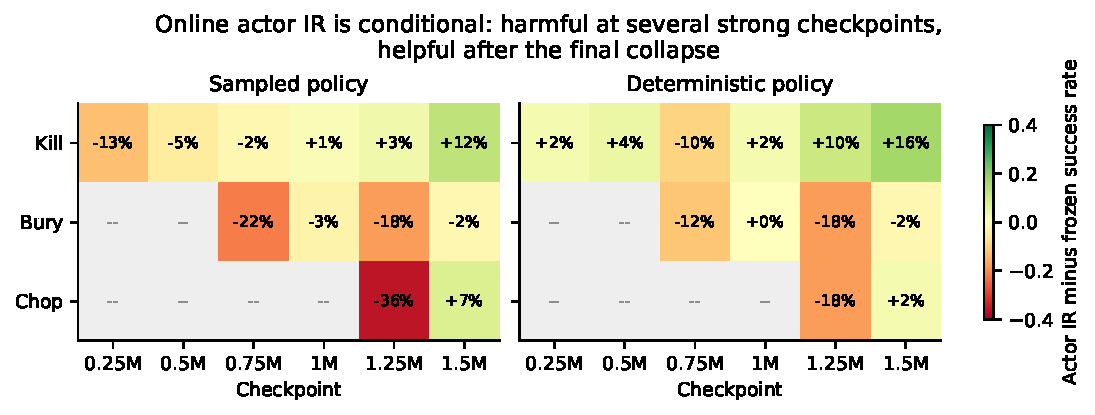
\includegraphics[width=.96\linewidth]{ir_delta_heatmaps.pdf}
\caption{IR effect in the reservoir run. Positive values mean actor-only IR improved success over the frozen checkpoint. Strong harm is concentrated at several high-performing checkpoint--goal pairs; final-checkpoint effects are small but consistently positive for kill and chop.}
\label{fig:irdelta}
\end{figure}

Across 24 mode-specific comparisons, IR improved 10, tied 1, and harmed 13. Averaged over all reservoir checkpoint--goal cells, sampled success fell from \pct{39.7} to \pct{33.2} ($-6.5$ points), while deterministic success fell from \pct{33.3} to \pct{31.3} ($-2.0$ points). The strongest harms were sampled chop at 1.25M ($-36$ points), sampled bury at 750k ($-22$), and both sampled and deterministic bury at 1.25M ($-18$).

At the final checkpoint---the most directly relevant corrupted-policy case---the pattern reversed. Mean sampled success rose from \pct{9.7} to \pct{15.3}, and deterministic success from \pct{11.3} to \pct{16.7}. Sampled kill improved from \pct{16} to \pct{28} (paired bootstrap 95\% interval for the 12-point change: $[2,23]$ points); chop improved from \pct{5} to \pct{12}; bury fell from \pct{8} to \pct{6}. Deterministic kill improved from \pct{24} to \pct{40}, although its 50-episode interval was wide ($[-4,36]$ points).

\begin{figure}[H]
\centering
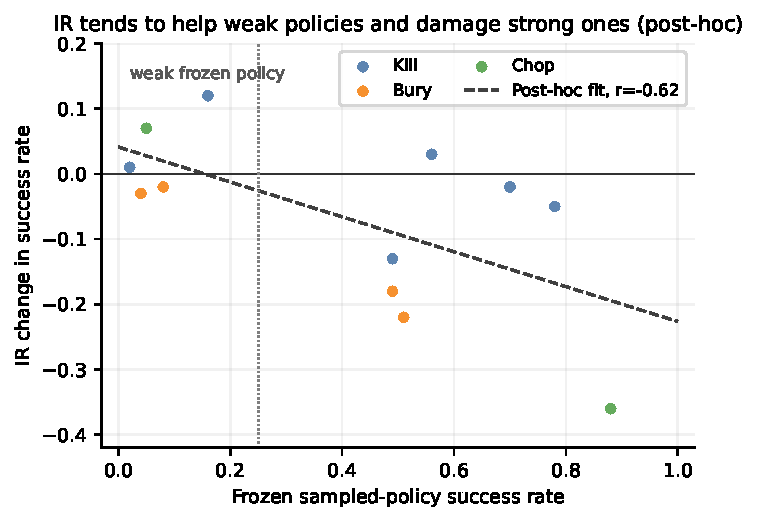
\includegraphics[width=.76\linewidth]{ir_strength_scatter.pdf}
\caption{Post-hoc relationship between frozen policy strength and sampled-policy IR effect. The correlation is $r=-0.50$. For cells with frozen success at most \pct{25} ($n=10$), mean IR effect was $+3.3$ points and six improved; above \pct{25} ($n=14$), mean effect was $-9.6$ points. This threshold was selected after seeing the data and is a hypothesis for a future gate, not a confirmatory result.}
\label{fig:irscatter}
\end{figure}

The negative association supports the original intuition behind gated IR: adapt when the actor appears damaged, and avoid perturbing a competent policy. It does not validate entropy as the gate variable, because this experiment did not record or intervene on a prespecified entropy threshold. Entropy also remained in the IR objective and may have dominated short-horizon updates in some states.

\begin{figure}[H]
\centering
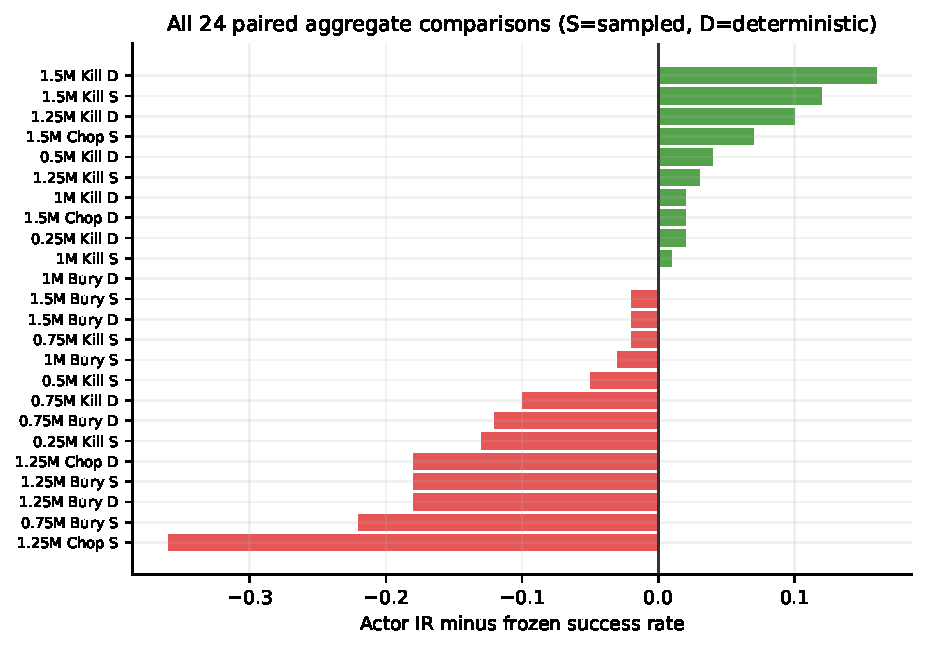
\includegraphics[width=.86\linewidth]{ir_all_conditions.pdf}
\caption{Every reservoir IR comparison, sorted by effect. S and D denote sampled and deterministic evaluation. The distribution is visibly asymmetric: a few large harms dominate several modest gains.}
\label{fig:irall}
\end{figure}

\begin{table}[H]
\centering
\caption{Aggregate success rates. Values are unweighted means over available checkpoint--goal cells.}
\label{tab:aggregate}
\begin{tabular}{llrrr}
\toprule
Replay & Policy mode & Frozen & Actor IR & IR change \\
\midrule
FIFO & Sampled       & 0.650 & 0.620 & $-0.030$ \\
FIFO & Deterministic & 0.648 & 0.623 & $-0.025$ \\
Reservoir & Sampled       & 0.397 & 0.332 & $-0.065$ \\
Reservoir & Deterministic & 0.333 & 0.313 & $-0.020$ \\
\midrule
Reservoir, final only & Sampled       & 0.097 & 0.153 & $+0.056$ \\
Reservoir, final only & Deterministic & 0.113 & 0.167 & $+0.053$ \\
\bottomrule
\end{tabular}
\end{table}

\section{Study I interpretation}

\subsection{What reservoir replay did establish}

The experiment rules out the claim that old-task data are wholly inaccessible under the new workflow. All goal strata were full, goal sampling was balanced, and earlier policies recovered sharply during chop training: from 1.0M to 1.25M, sampled kill rose from \pct{2} to \pct{56}, bury from \pct{4} to \pct{49}, while chop reached \pct{88}. That combination would be very unlikely if replay groups, reset boundaries, goal IDs, or head conditioning were completely broken.

The experiment does \emph{not} prove that the reward model and critic are well calibrated for every goal. Behavioral success is an end-to-end diagnostic. A model can contain enough signal for recovery while still having biased reward predictions, value misranking, or compounding imagination error. Direct head-calibration probes remain necessary.

\subsection{Why balanced replay may still collapse}

Several mechanisms are consistent with the observed synchronized swings:
\begin{enumerate}
  \item \textbf{Optimization interference.} Shared encoder, RSSM, and large actor receive gradients induced by multiple visually similar but behaviorally distinct goals. Balanced data availability does not guarantee compatible gradients.
  \item \textbf{Reduced current-task dose.} Once three strata exist, only about one third of replay batches target the active goal, while the nominal training ratio remains fixed. The reservoir condition is not update-dose matched to FIFO.
  \item \textbf{Episode-uniform versus transition-uniform sampling.} Complete-episode selection changes the weight of short successful and long failed episodes relative to FIFO sequence-start sampling.
  \item \textbf{Head/world-model drift.} The RSSM is goal-agnostic and shared. Even if every goal is represented in replay, representation changes can move the inputs seen by reward, value, and actor heads.
  \item \textbf{Single-run stochasticity.} With one seed, a late policy collapse cannot yet be separated from an unlucky optimization trajectory.
\end{enumerate}

The result therefore argues for measuring subsystem health, not merely increasing replay capacity.

\subsection{Why ungated IR can hurt}

IR trusts imagined returns. When the actor is already competent, one update at every real action creates many opportunities to move away from a successful action mode because of value error, model exploitation, posterior sampling noise, or the entropy term. A six-step horizon reduces compounding error but does not eliminate it. Conversely, a badly damaged actor has more room for improvement, which matches the final-checkpoint recovery and the post-hoc negative correlation in Figure~\ref{fig:irscatter}.

The next IR study should therefore begin with a controlled actor-corruption experiment: choose a checkpoint with high task success and intact goal-conditioned heads, perturb only the actor to known severity levels, and measure recovery under frozen versus adapted actors. That design isolates whether IR can repair policy damage when its model and critic are known to be competent.

\section{Study I limitations and threats to validity}

\begin{itemize}
  \item \textbf{One seed.} All uncertainty intervals quantify episode-level evaluation variability, not training-seed variability. They must not be interpreted as generalization across runs.
  \item \textbf{Replay conditions are not capacity matched.} FIFO capacity is counted in sequence starts; reservoir capacity is counted in complete episodes and consumed more host memory.
  \item \textbf{Optimization exposure differs.} Goal-balanced sampling necessarily decreases the current task's fraction as goals accumulate. A fair algorithmic ablation may need either ratio compensation or a tunable current/old mixture.
  \item \textbf{Evaluation pairing is imperfect.} Seed and goal schedules match, but separate process lifetimes produced different initial frame hashes. Episode-order paired bootstrap intervals \citep{efron1993bootstrap} are informative, not exact paired-environment causal estimates.
  \item \textbf{FIFO summaries are legacy artifacts.} The old evaluation supervisor marked the queue failed under a subsequently fixed frame-hash rule. Completed first-attempt summaries are retained for descriptive comparison.
  \item \textbf{No direct model calibration.} Reward-head accuracy, value calibration, imagined-return bias, and goal separability were not measured. Behavioral success alone cannot locate the failing subsystem.
  \item \textbf{Post-hoc gate analysis.} The \pct{25} frozen-performance split and its correlation were discovered after observing outcomes. A future run must prespecify and validate any gate.
  \item \textbf{Environment scope.} The three chosen tasks use the same 504-way click grid and are solvable with left clicks. Results need not transfer to the two harder RLScape goals or to continuous robotic control.
\end{itemize}

\section{Decision point after Study I}

The checkpoint archive makes the following sequence possible without immediately repeating the multi-day run:

\begin{enumerate}
  \item \textbf{Head audit at strong and collapsed checkpoints.} For a fixed image/latent set, measure goal-conditioned reward prediction, continuation, value ranking, and imagined-versus-real return. Include wrong-goal counterfactuals to quantify whether $g$ changes the heads functionally.
  \item \textbf{Actor corruption and recovery.} Start from the strongest checkpoint for each goal; apply controlled actor noise or partial reinitialization; compare frozen, ungated IR, IR without entropy, and IR with smaller learning rates/horizons.
  \item \textbf{Prespecified IR gate.} Gate on a measurable signal available at test time---for example ensemble disagreement, low predicted value relative to a checkpoint baseline, or sustained high entropy. Entropy alone should be treated as one candidate, not an assumption.
  \item \textbf{Replay-mixture ablation.} Keep Algorithm R retention but compare uniform goal sampling with a current-goal-biased mixture, such as 50\% current and 50\% uniformly old. Match total update dose where possible.
  \item \textbf{Stability replication.} Repeat the best replay/IR configuration over multiple seeds, then extend from three to all five RLScape goals.
  \item \textbf{Return phase.} Finally revisit $A$ after $A\rightarrow B\rightarrow C$ to quantify relearning speed, forward/backward transfer, and whether IR reduces real-environment samples.
\end{enumerate}

Hindsight relabeling remains a possible later extension for sparse rewards, but it is not the first diagnosis: all three tasks already reached near-perfect training windows, so the immediate bottleneck is maintaining and exploiting learned competence.

\section{Interim conclusion after Study I}

The reservoir implementation worked, the long-running workflow was operationally robust, and every task was individually learnable inside the sequential run. Yet goal-stratified reservoir replay did not solve continual learning by itself. It produced compelling but temporary balanced retention, then ended in a synchronized behavioral collapse substantially worse than FIFO's final mean. Actor-only IR was also not uniformly beneficial: fixed every-action updates often damaged strong actors, while providing modest recovery at the final weak checkpoint.

The most useful outcome is therefore diagnostic. Old experience and goal-conditioned knowledge can support recovery, but neither balanced replay nor ungated test-time adaptation guarantees stability. The next experiments should exploit the saved checkpoints to separate actor damage from reward/value/world-model failure and to design an IR gate before spending another multi-day training budget.

\section{Study II: locating the failure inside the learned IR target}

Study I left an ambiguity that could not be resolved from behavioral success alone. A weak actor may fail because the policy parameters are damaged while the world model, reward head, continuation head, and critic remain useful. Alternatively, the actor may be reacting rationally to an inaccurate learned objective. This distinction is decisive for IR: test-time actor optimization is only useful when the frozen components supply a trustworthy teaching signal.

Study II therefore compares the \textbf{strong 1.25M checkpoint} with the \textbf{collapsed 1.5M checkpoint}. At 1.25M, sampled-policy success was \pct{56}/\pct{49}/\pct{88} on kill/bury/chop. At 1.5M, every task was at most \pct{16}, with a mean of \pct{9.7}. The analysis has two linked parts. Study IIa evaluates the learned heads on real replay trajectories. Study IIb executes the exact actor-IR imagination path, without updating parameters, to measure where its return and gradient signals originate.

\subsection{Study IIa method: immutable same-state head audit}

The state bank was drawn from the pinned 1.25M replay archive, not recollected separately under each checkpoint. For every trained goal it contains 64 successful and 64 failed episodes, yielding 384 episodes and 48,299 states. Both checkpoints therefore receive the same image sequences, actions, reset boundaries, rewards, continuations, and factual goal labels. This design removes changes in environment sampling from the strong--weak comparison.

Each sequence is encoded under each checkpoint to obtain its posterior latent trajectory. At every state, the reward, continuation, online value, and slow-value heads are queried under all five one-hot goal IDs: the three trained goals and the unused \emph{light fire} and \emph{catch fish} slots. ``Factual'' means the goal used when that replay episode was collected. ``Counterfactual'' means that the latent state and every other input are held fixed while only the one-hot goal is changed.

For reward and continuation, the most important counterfactual query is a completion state for goal $i$ evaluated under another goal $j\neq i$. The desired targets are
\begin{align}
  r(s^{\mathrm{complete}(i)},g_i)&=1, &
  c(s^{\mathrm{complete}(i)},g_i)&=0,\\
  r(s^{\mathrm{complete}(i)},g_j)&=0, &
  c(s^{\mathrm{complete}(i)},g_j)&=1 \quad (j\neq i).
  \label{eq:counterfactualtargets}
\end{align}
The second line was never supplied by ordinary on-policy replay: every observed completion appears only with its active goal. The audit measures whether one-hot conditioning nevertheless induced that semantic distinction.

Value calibration compares predicted values with recorded discounted returns along the replay trajectory. This is a diagnostic rather than an exact reconstruction of Dreamer's critic loss: replay actions are off-policy relative to each audited checkpoint, whereas Dreamer trains lambda returns under imagined policy rollouts. The comparison remains valuable because both checkpoints are evaluated on identical states, empirical returns remain in $[0,1]$, and the strong-to-weak direction can be compared directly. Parameter digests before and after both audits are identical.

\subsection{Study IIa results: event recognition without goal semantics}

\paragraph{Factual reward prediction remains excellent.}
Reward AUROC is 0.99993 at 1.25M and 0.99991 at 1.5M. Mean reward prediction on genuine completion states is 0.961 and 0.957, while ordinary-state false positives remain very small. Thus replay retention preserved a highly accurate detector of visible completion-like events through the behavioral collapse.

\paragraph{The reward head scarcely uses the requested goal.}
On the same completion states, the factual-minus-counterfactual reward margin is only 0.0033 at 1.25M and 0.0018 at 1.5M. Choosing the goal with the largest reward prediction identifies the correct goal only \pct{39.6} and \pct{38.0} of the time despite five goal slots. The head has learned ``a task completed'' much more strongly than ``the requested task completed.''

\paragraph{Continuation has the same semantic failure.}
The continuation head accurately predicts stopping on factual completion states and continuing on ordinary states. Yet mean stop probability on wrong-goal completion queries is already \pct{93.9}/\pct{94.3} at the strong/weak checkpoint, compared with only \pct{95.6}/\pct{95.9} for the matching goal. Reward and continuation are therefore separate heads but share the same missing counterfactual supervision.

\begin{figure}[H]
\centering
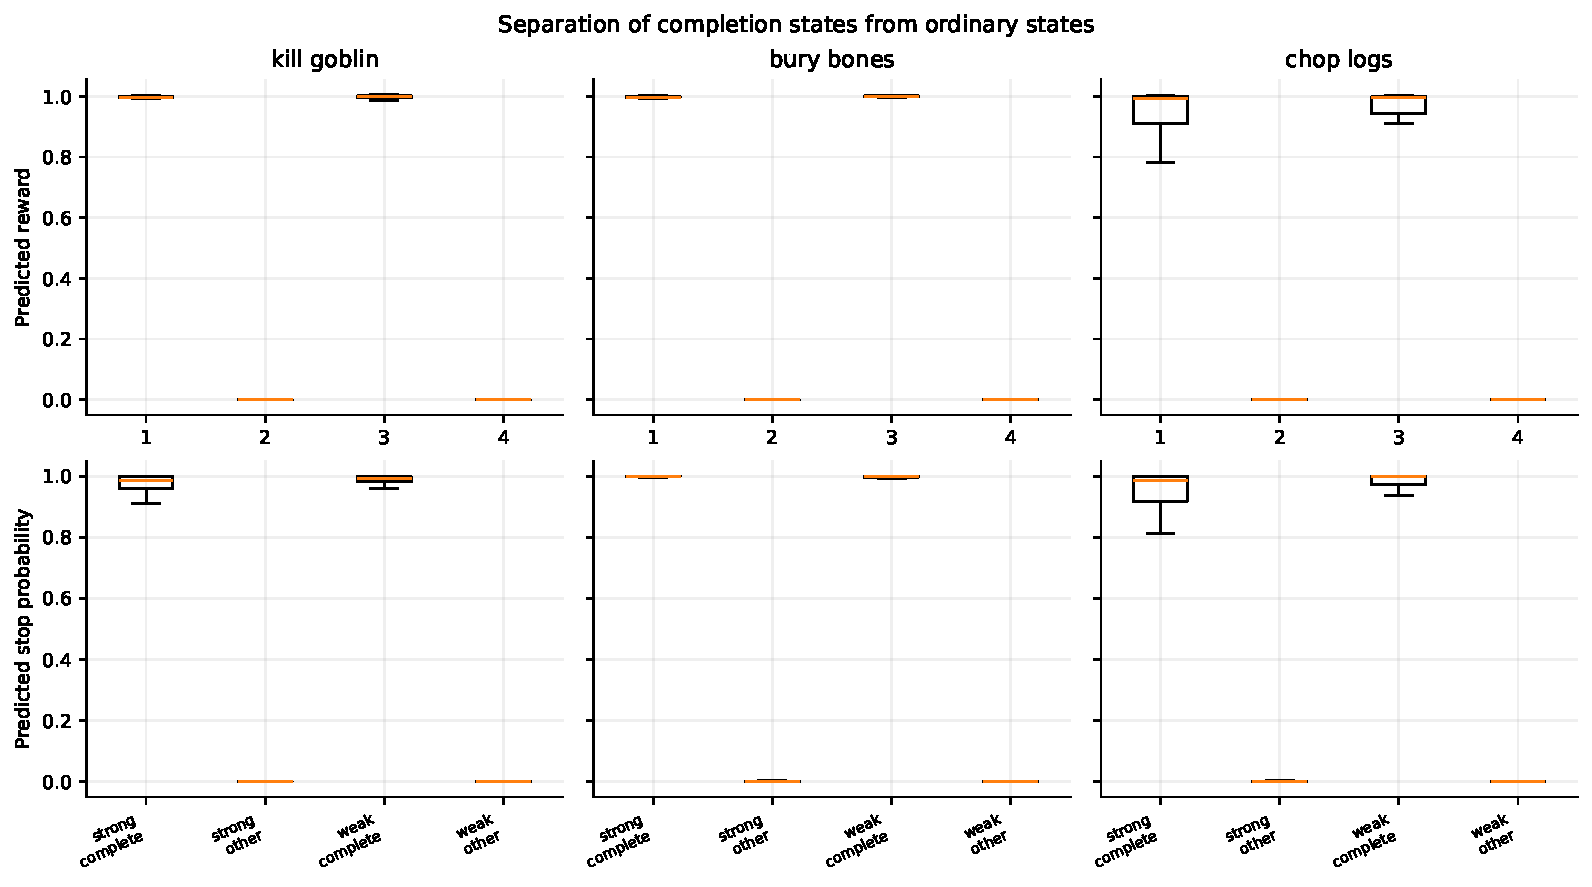
\includegraphics[width=.98\linewidth]{stage1a_same_state_head_audit/head_separation.pdf}
\caption{Study IIa factual event recognition. Reward (top) and stopping (bottom) almost perfectly separate completion states from ordinary states at both checkpoints. This figure is deliberately paired with the counterfactual analysis: factual accuracy alone can hide the fact that the same completion state receives almost the same output under every requested goal.}
\label{fig:stage1heads}
\end{figure}

\paragraph{The critic is severely overoptimistic and worsens after collapse.}
At 1.25M, mean factual critic predictions are 1.62, 1.73, and 0.79 for kill, bury, and chop, whereas empirical discounted-return means are 0.20, 0.10, and 0.21. At 1.5M, values rise further to 1.99, 2.00, and 1.36 even though real policy success collapses. Value--return Pearson correlations deteriorate from 0.182/0.107/0.307 to 0.048/0.064/0.061. At episode starts, value barely separates successful from failed kill trajectories, reverses their ordering for bury, and weakens for chop.

\begin{figure}[H]
\centering
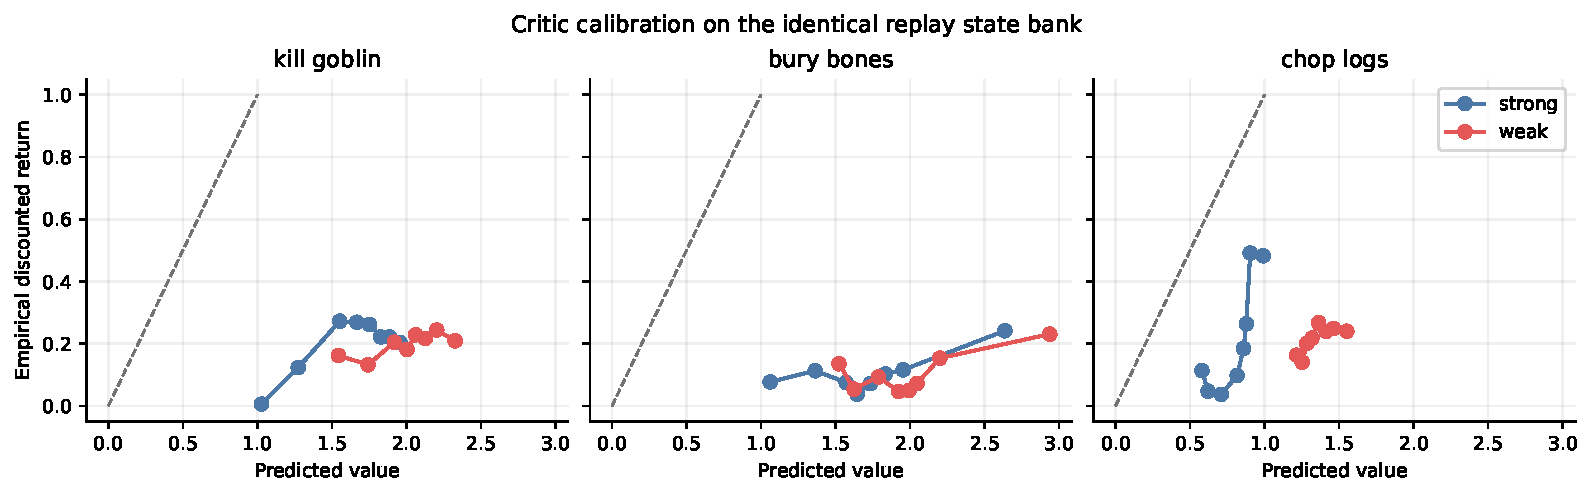
\includegraphics[width=.98\linewidth]{stage1a_same_state_head_audit/value_calibration.pdf}
\caption{Study IIa critic calibration on the identical replay-state bank. The dashed line is ideal calibration. Predicted values are far above recorded discounted returns, and the weak checkpoint (red) is generally more optimistic despite much worse real behavior.}
\label{fig:stage1valuecal}
\end{figure}

The slow critic does not provide an independent safety signal. Its mean absolute disagreement with the online critic is only 0.006--0.017; both share the same optimism and drift. Posterior categorical entropy changes only from 0.564 to 0.543 and deterministic-state RMS from 0.256 to 0.262. These scalar summaries do not rule out task-relevant representation drift, but they rule out a gross posterior entropy or magnitude collapse as the immediate explanation.

\begin{figure}[H]
\centering
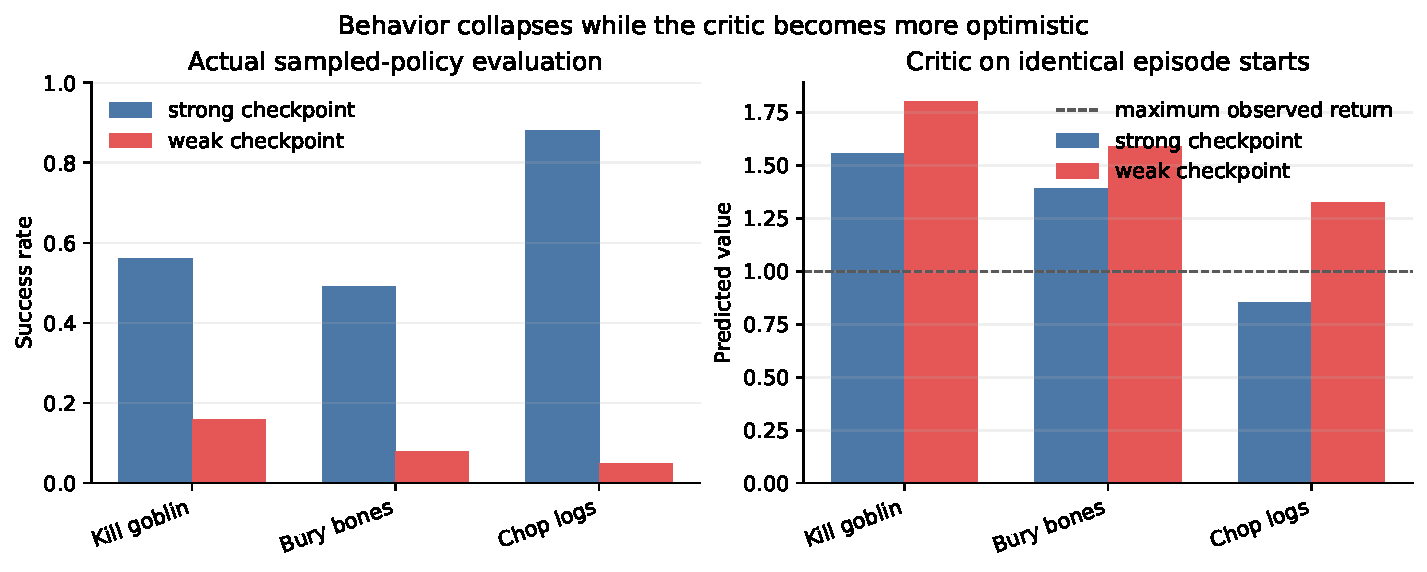
\includegraphics[width=.94\linewidth]{stage1a_same_state_head_audit/behavior_vs_critic.pdf}
\caption{Behavior and critic confidence move in opposite directions between the strong and weak checkpoints. This inverse relationship motivated an audit of the exact imagined return used by actor IR rather than treating critic output as a valid gate.}
\label{fig:behaviorcritic}
\end{figure}

\subsection{Study IIb method: exact six-step imagination-path audit}

Study IIb reuses the same 384-episode selection. Four deterministic, nonterminal anchors are requested from each episode; short trajectories yield 1,433 valid anchors. At every anchor, the agent reconstructs the posterior latent state and sweeps all five goal IDs. For each anchor--goal pair, it draws 128 paired posterior samples and executes the same $H=6$ policy imagination used by Study I actor IR. In total, each checkpoint produces 7,165 anchor--goal rollouts and 5,502,720 imagined action transitions.

No optimizer update is applied. Instead, the audit records, at each imagined time step:
\begin{itemize}
  \item predicted reward and the incidence of reward-like events;
  \item continuation and predicted stopping events;
  \item online and slow critic values;
  \item lambda return, split into reward-only and critic-bootstrap contributions;
  \item actor reinforce/advantage term, entropy term, and policy entropy;
  \item actual replay goal, probed goal, anchor location, and success/failure stratum.
\end{itemize}
Randomness is paired across goal probes so differences are attributable to the one-hot goal rather than different posterior samples. Parameter digests again match before and after the audit.

For clarity, write the imagined truncated return abstractly as
\begin{equation}
  \widehat G^{\lambda,H}_t
  = \underbrace{\sum_{k=0}^{H-1} w_{t,k}\hat r_{t+k}}_{\text{reward contribution}}
  + \underbrace{b_{t,H}\,v_{\bar\psi}(\hat s_{t+H},g)}_{\text{critic bootstrap}},
  \label{eq:decomp}
\end{equation}
where the actual implementation uses Dreamer's lambda-return weighting and continuation discounts. The audit reconstructs both contributions rather than inferring them from the total.

\subsection{Study IIb results: IR optimizes the critic, not imagined reward}

\paragraph{Critic bootstrap dominates the IR target.}
At the strong checkpoint, mean factual lambda return is 1.450: only 0.072 is attributable to imagined rewards and 1.378 to bootstrap, a \pct{94.4} bootstrap fraction. At the weak checkpoint, mean return rises to 1.868 despite behavioral collapse: reward contribution falls to 0.039 while bootstrap rises to 1.829, or \pct{97.3}. Ordinary anchors are more than \pct{99} bootstrap driven. Even immediately before recorded completion, bootstrap still contributes \pct{69.1} at the strong checkpoint and \pct{82.4} at the weak checkpoint.

\begin{figure}[H]
\centering
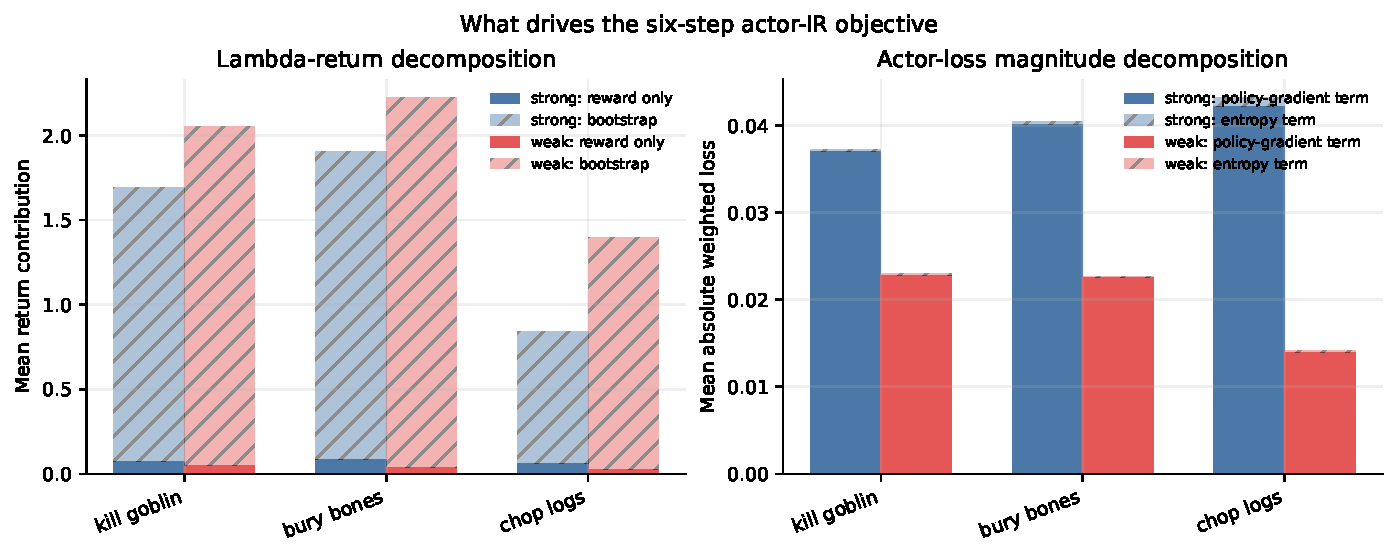
\includegraphics[width=.98\linewidth]{stage1b_imagination_path_audit/ir_objective_decomposition.pdf}
\caption{Study IIb decomposition of the exact six-step actor-IR objective. Left: lambda return is almost entirely critic bootstrap, and bootstrap grows at the weak checkpoint while imagined reward shrinks. Right: entropy is small relative to the policy-gradient term in measured scalar loss magnitude.}
\label{fig:objectiveparts}
\end{figure}

\paragraph{The weak model imagines fewer successes but larger returns.}
Factual imagined reward-event incidence falls from \pct{6.76} to \pct{3.52} of MCPB posterior samples, and reward-only return falls from 0.072 to 0.039. Nevertheless, bootstrap increases by 0.451 and total return increases by 0.419. Factual starting value rises from 1.315 to 1.668. The optimism observed on replay states is therefore present on the exact IR path and overwhelms the direction of the reward evidence.

\paragraph{Goal identity scarcely changes the teaching signal.}
Strong-checkpoint factual and counterfactual imagined returns are 1.450 and 1.447. At the weak checkpoint they are 1.868 and 1.865. On pre-completion anchors, factual versus wrong-goal reward-event rates are \pct{34.0} versus \pct{33.5} at 1.25M and \pct{21.2} versus \pct{20.8} at 1.5M. Requested-goal top-1 identification from imagined return degrades from \pct{52.8} to \pct{41.9}, and the factual-minus-wrong-goal mean margin is only 0.0029/0.0032.

\begin{figure}[H]
\centering
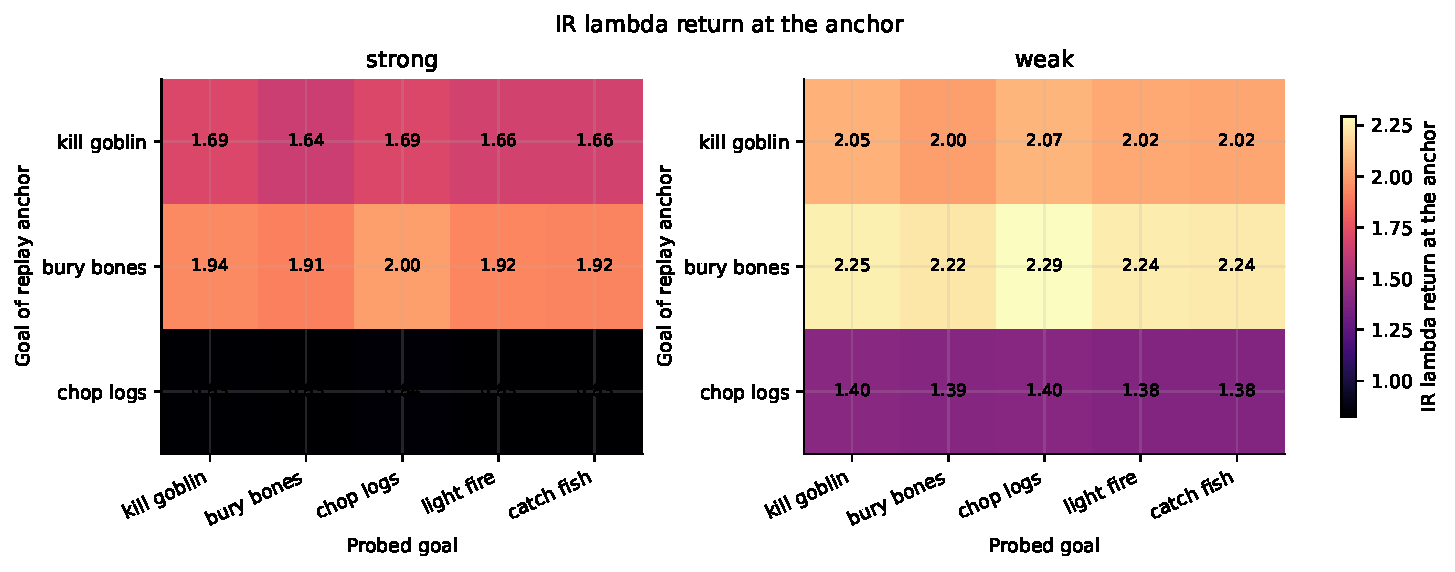
\includegraphics[width=.94\linewidth]{stage1b_imagination_path_audit/imagined_return.pdf}
\caption{Mean IR lambda return by replay anchor goal (rows) and requested one-hot goal (columns). Row identity dominates column identity: the source trajectory matters far more than the goal requested for rehearsal. The weak checkpoint is uniformly more optimistic.}
\label{fig:imagreturn}
\end{figure}

Reward and stopping events remain meaningful visual detectors: on successful trajectories, factual imagined reward-event incidence is \pct{12.5} (strong) and \pct{6.7} (weak), versus \pct{1.8} and \pct{0.7} on failed trajectories. Events concentrate near factual pre-completion states. The defect is not absence of all model signal; it is the missing same-state, wrong-goal distinction.

\paragraph{Entropy is not the dominant scalar term.}
Mean absolute factual policy-gradient loss is 0.0398 at 1.25M and 0.0196 at 1.5M. The corresponding entropy terms are 0.000552 and 0.000180, approximately \pct{1.4} and \pct{0.9} of those aggregate magnitudes; mean per-rollout ratios are \pct{2.2} and \pct{1.6}. These are scalar loss comparisons rather than gradient-norm comparisons, so an entropy ablation remains justified. They do not, however, support entropy as the primary explanation.

The actor itself becomes much more deterministic after collapse: factual policy entropy falls from 1.915 to 0.628. Simultaneously, the mean absolute policy-gradient term approximately halves. In other words, the damaged policy has less exploratory diversity while the learned objective intended to repair it becomes less informative and more bootstrap dominated.

\subsection{Study II interpretation and resulting prediction}

The two audits form a consistent mechanism. Reservoir replay preserved factual examples, so reward and continuation learned excellent visual event detection. It did not create the counterfactual labels in Equation~\ref{eq:counterfactualtargets}; those heads can minimize factual loss while almost ignoring $g$. The critic then bootstraps on its own predictions through imagined states and develops values that are both too large and increasingly detached from realized success. Standard actor IR mostly optimizes this critic bootstrap.

This does not by itself prove the ultimate origin of critic optimism. Plausible contributors include self-reinforcing bootstrap targets, distribution shift into policy-imagined states, exploitation of model errors, weak goal selectivity, and continual drift in shared representations. What Study II establishes more narrowly is that \emph{the critic is not a trustworthy teacher for the next actor-recovery experiment}. It therefore made a falsifiable prediction: if actor adaptation is mechanically viable, removing critic bootstrap should outperform standard IR; removing entropy alone should not.

\section{Study III: controlled actor corruption and recovery}

\subsection{Question and experimental controls}

Study III asks whether actor-only imagined adaptation can recover a deliberately damaged policy when every non-actor component is held fixed. It is a mechanism experiment, not another continual-training run. The source is the pinned 1.25M checkpoint, chosen because all three goals were simultaneously competent and Study II had already characterized its heads and imagination path.

The experiment applies an independent zero mask to actor parameters only. Encoder, RSSM, decoder, reward, continuation, online value, slow value, normalizers, and their optimizer states remain byte-identical to the source. Six mask probabilities, $p\in\{0.1,0.2,0.3,0.4,0.5,0.6\}$, are calibrated on 20 sampled episodes per goal using paired reset seeds. The selection target is \pct{35} aggregate retention of clean success, accepted only within \pct{10}--\pct{65}, with no goal retaining more than \pct{85} and a penalty for uneven or beneficial corruption.

The selected 40\% zero mask affects all 11 actor parameter arrays (3,409,912 parameters) and has actor-relative $L_2$ distance 0.637 from the source, close to the $\sqrt{0.4}$ scale expected for independent masking. In calibration it retains \pct{35.1} of aggregate clean success: per-goal retention is \pct{50.0}, \pct{20.0}, and \pct{35.3} for kill, bury, and chop. The independent main seed schedule produces a less severe but still substantial sampled decline, from \pct{56.3} clean mean to \pct{28.3} corrupted mean.

\begin{figure}[H]
\centering
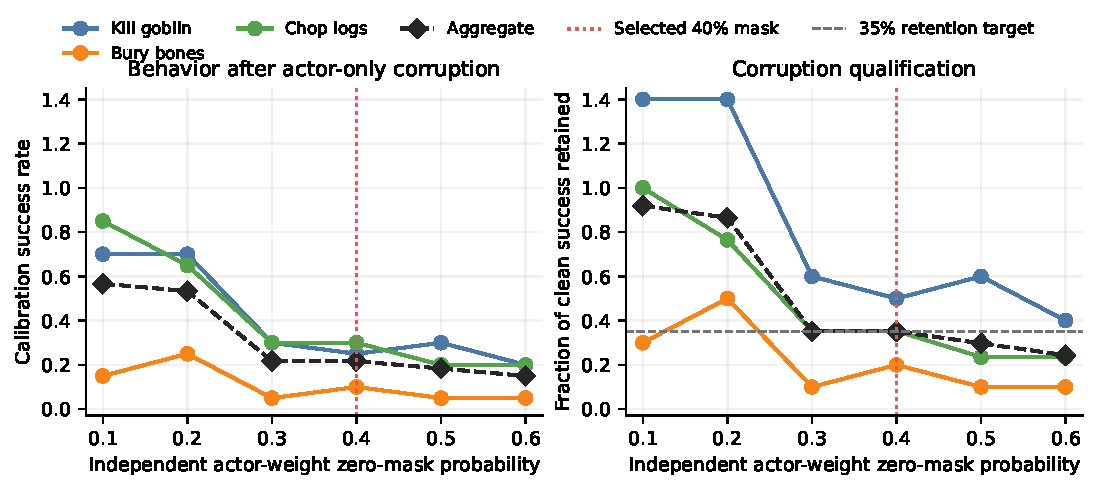
\includegraphics[width=.96\linewidth]{stage2_controlled_actor_recovery/corruption_calibration.pdf}
\caption{Study III corruption calibration. Six actor-only mask strengths were evaluated before the main assay. The 40\% mask is the qualified candidate closest to the prespecified \pct{35} aggregate-retention target while avoiding near-intact individual goals.}
\label{fig:corruptcal}
\end{figure}

Every evaluation episode begins from the same persistent checkpoint parameters. Temporary actor parameters adapt from the first real posterior state and then once per environment action; they accumulate within the episode and are discarded at reset. Each update uses 128 posterior samples, learning rate $4\times10^{-5}$, and one optimizer step. The world model and both critics are frozen in every arm. Horizons are $H\in\{3,6,15,20\}$.

\subsection{Recovery objectives}

Fifteen conditions separate three possible causes of failure.

\paragraph{No-adaptation controls.}
The clean and corrupted actors establish the attainable source behavior and the size of the induced deficit under the same main evaluation schedule.

\paragraph{Standard IR.}
This is the learned Dreamer actor objective used in Study I: policy gradients from normalized imagined lambda returns, including value bootstrap, plus entropy coefficient $3\times10^{-4}$. It is tested at all four horizons.

\paragraph{Entropy-off standard IR.}
This arm keeps the standard imagined return and critic bootstrap but sets the entropy coefficient to zero. It directly tests whether entropy, rather than the return target, caused harmful updates.

\paragraph{Reward-only IR.}
This arm uses predicted reward and continuation along the imagined rollout but sets terminal value bootstrap and entropy to zero. Abstractly,
\begin{equation}
  J_{\mathrm{RO}}(\theta;s,g)
  =\mathbb E_{p_\phi,\pi_\theta}
    \left[\sum_{k=0}^{H-1}\left(\prod_{j<k}\hat c_{t+j}\right)
    \gamma^k\hat r_{t+k}\right],
  \label{eq:rewardonly}
\end{equation}
with the implementation retaining Dreamer's differentiable policy-gradient machinery and giving posterior samples whose imagined trajectories contain zero reward no policy-gradient signal. This is a diagnostic critic-free objective, not an oracle: rewards and continuations are still learned model predictions.

\paragraph{Clean-reference distillation.}
The frozen clean actor supplies its full categorical action distribution on the current real posterior state. The temporary corrupted actor minimizes cross-entropy to that teacher. This horizon-independent positive control tests whether the corruption can be reversed under the same episode-local actor optimizer without relying on imagined returns.

\subsection{Evaluation scale and integrity}

Every condition is evaluated on all three goals with 100 sampled and 50 deterministic episodes. The main matrix therefore contains
\begin{equation}
  15\text{ conditions}\times3\text{ goals}\times(100+50)
  =6{,}750\text{ real-environment episodes}.
\end{equation}
Calibration contributes 420 further episodes. In runner terms, all 21 calibration units and all 90 main units completed, giving 111 complete units with no failed attempt or retry. Goal, policy mode, and reset-seed identities match across conditions; the pairing audit reports no mismatch. Requested episode counts, reset counts, return codes, and persistent parameter-integrity digests all pass.

\subsection{Study III results}

\begin{figure}[H]
\centering
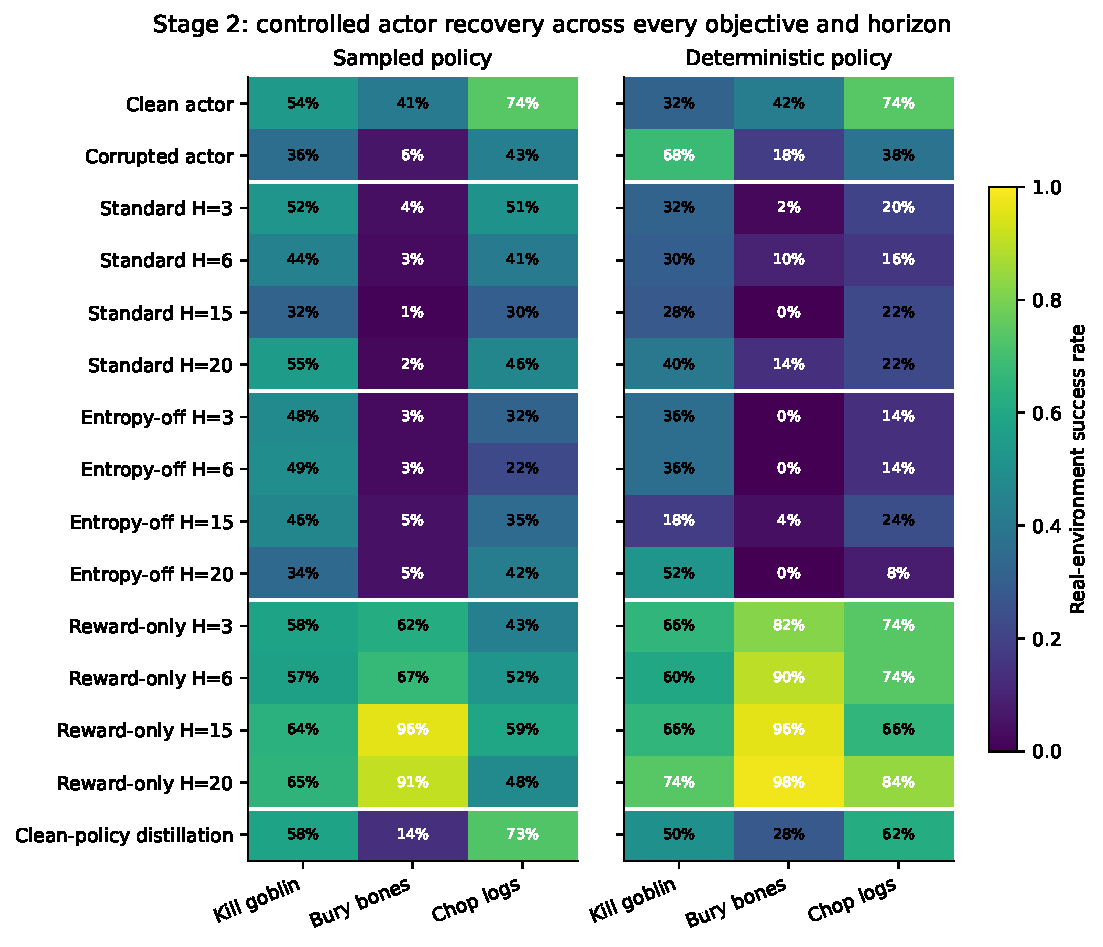
\includegraphics[width=.98\linewidth]{stage2_controlled_actor_recovery/condition_matrix.pdf}
\caption{Complete Study III result matrix. Each cell is real-environment task success, not predicted reward. Standard and entropy-off IR remain weak, while reward-only IR recovers the actor and often exceeds the clean source behavior.}
\label{fig:stage2matrix}
\end{figure}

\begin{table}[H]
\centering
\small
\caption{Aggregate Study III success across all three goals. Sampled totals use 300 episodes per row; deterministic totals use 150. ``Best'' selects the horizon separately within each objective family and policy mode.}
\label{tab:stage2aggregate}
\begin{tabular}{lrrl}
\toprule
Condition & Sampled mean & Deterministic mean & Interpretation \\
\midrule
Clean actor & .563 & .493 & Source checkpoint \\
Corrupted actor & .283 & .413 & Actor-only deficit \\
Standard IR, best & .357 ($H=3$) & .253 ($H=20$) & Weak sampled; destructive deterministic \\
Entropy-off IR, best & .287 ($H=15$) & .200 ($H=20$) & Removing entropy does not repair IR \\
Reward-only IR, $H=3$ & .543 & .740 & Near/full aggregate recovery \\
Reward-only IR, $H=6$ & .587 & .747 & Exceeds clean mean \\
Reward-only IR, $H=15$ & \textbf{.730} & .760 & Best sampled result \\
Reward-only IR, $H=20$ & .680 & \textbf{.853} & Best deterministic result \\
Clean-policy distillation & .483 & .467 & Partial positive-control recovery \\
\bottomrule
\end{tabular}
\end{table}

\paragraph{Standard IR is narrow and unstable.}
At $H=3$, sampled kill improves from \pct{36} to \pct{52} and chop from \pct{43} to \pct{51}, but bury remains near zero. Aggregate sampled success rises only to \pct{35.7}. At $H=6$ it falls to \pct{29.3}; at $H=15$ it drops below the corrupted baseline to \pct{21.0}; at $H=20$ it rebounds to \pct{34.3}. Deterministic success is damaged at every horizon, ranging from \pct{16.7} to \pct{25.3} versus \pct{41.3} corrupted. Standard IR can discover a useful local direction for one policy/task combination, but its teaching signal is not robust.

\paragraph{Entropy removal does not solve the failure.}
Entropy-off sampled means remain between \pct{24.7} and \pct{28.7}; deterministic means remain between \pct{15.3} and \pct{20.0}. This agrees with Study IIb's objective decomposition. Entropy may influence individual decisions, but it is neither necessary nor sufficient for the broad harm.

\paragraph{Removing critic bootstrap changes the outcome decisively.}
Reward-only IR reaches sampled means of \pct{54.3}, \pct{58.7}, \pct{73.0}, and \pct{68.0} as $H$ increases from 3 to 20. Deterministic means are \pct{74.0}, \pct{74.7}, \pct{76.0}, and \pct{85.3}. The result is not merely recovery to the clean actor: the best reward-only conditions exceed it by 16.7 sampled points and 36.0 deterministic points.

\begin{figure}[H]
\centering
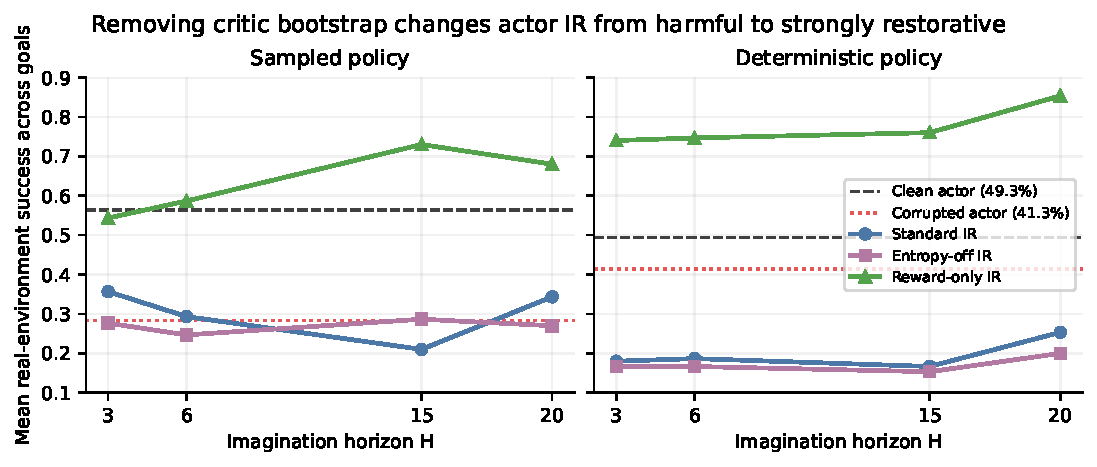
\includegraphics[width=.98\linewidth]{stage2_controlled_actor_recovery/horizon_aggregate.pdf}
\caption{Aggregate horizon response. Standard and entropy-off IR track the corrupted baseline or fall below it. Reward-only IR crosses the clean-actor line and generally benefits from longer imagination. This is the central causal ablation of the chapter.}
\label{fig:horizonaggregate}
\end{figure}

The per-goal pattern is informative. At sampled $H=15$, reward-only IR obtains \pct{64} kill, \pct{96} bury, and \pct{59} chop. Relative to paired corrupted episodes, changes are $+28$ points (95\% interval $[+15,+40]$), $+90$ $[+83,+96]$, and $+16$ $[+2,+30]$. All exclude zero. At $H=20$, corresponding changes are $+29$ $[+17,+41]$, $+85$ $[+77,+92]$, and $+5$ $[-8,+19]$. Thus $H=15$ is the most consistent sampled horizon; $H=20$ is strongest under deterministic action selection.

\begin{figure}[H]
\centering
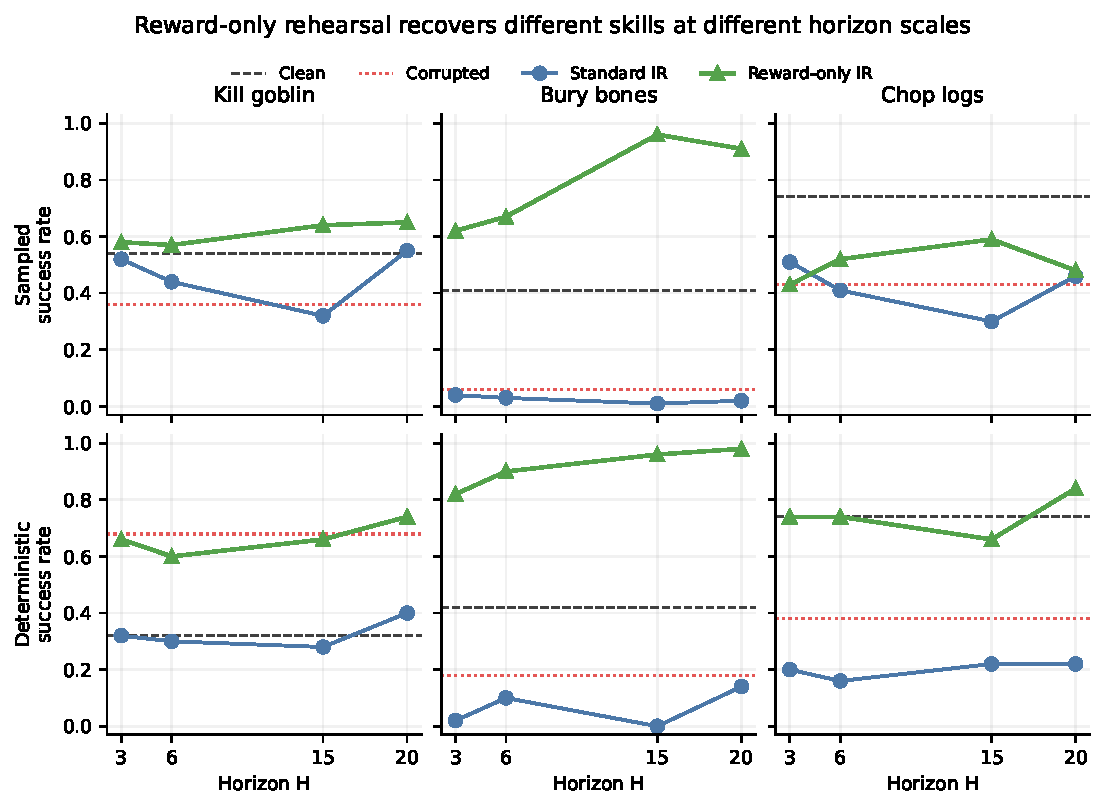
\includegraphics[width=.98\linewidth]{stage2_controlled_actor_recovery/reward_only_by_goal.pdf}
\caption{Goal-specific horizon response. Bury bones exhibits dramatic reward-only recovery, kill improves consistently under sampled control, and chop peaks earlier or weakens at sampled $H=20$. There is no single horizon that dominates every task and policy mode.}
\label{fig:stage2goals}
\end{figure}

\begin{figure}[H]
\centering
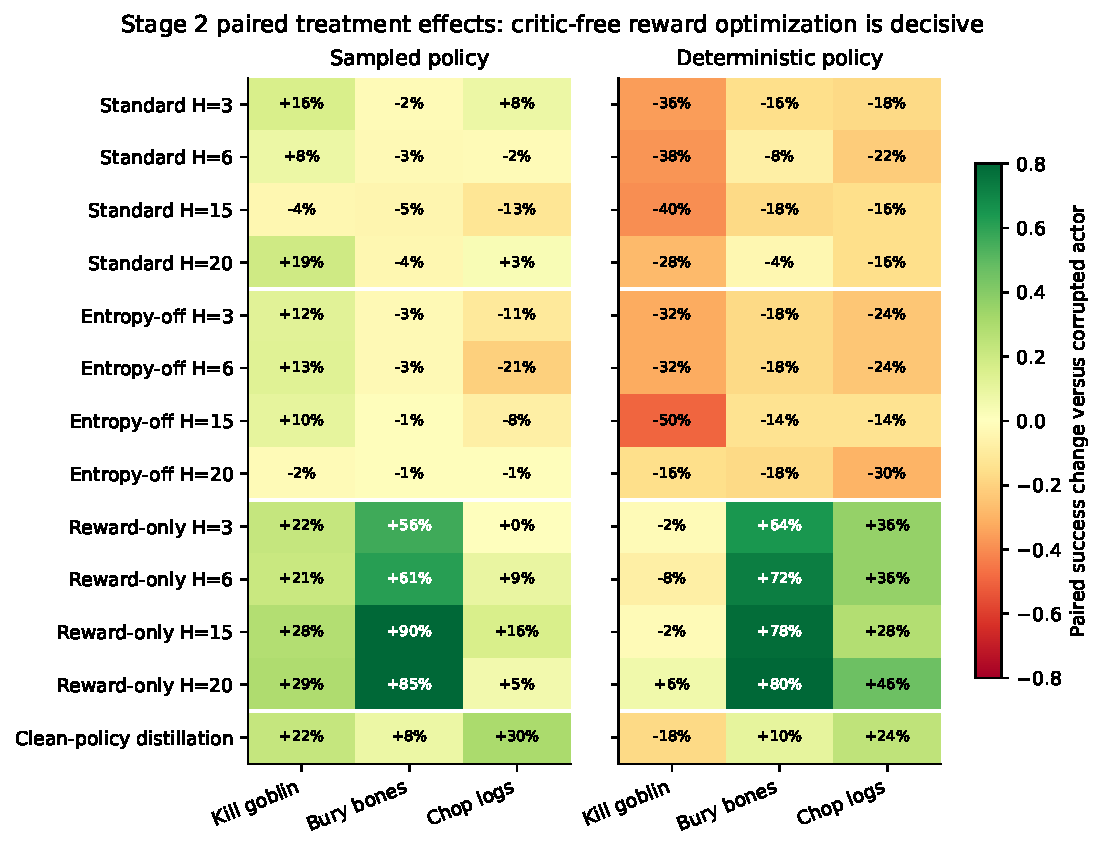
\includegraphics[width=.98\linewidth]{stage2_controlled_actor_recovery/paired_effects.pdf}
\caption{Paired changes relative to the corrupted actor. The green reward-only block contrasts sharply with standard and entropy-off objectives. Deterministic kill requires special caution because actor corruption itself improved its raw deterministic success from \pct{32} clean to \pct{68} corrupted.}
\label{fig:stage2effects}
\end{figure}

\paragraph{Reference distillation provides partial mechanical recovery.}
Distillation raises sampled aggregate success from \pct{28.3} to \pct{48.3}: kill rises \pct{36}$\rightarrow$\pct{58}, bury \pct{6}$\rightarrow$\pct{14}, and chop \pct{43}$\rightarrow$\pct{73}. It does not exactly recreate the source policy within the limited episode-local updates, especially on bury, but it confirms that the optimizer can move the corrupted actor toward a trusted target. Reward-only IR's much stronger bury result is therefore not explained by simple cloning of the original actor; it constitutes online policy improvement under the learned reward model.

\subsection{Study III interpretation}

Study III supports the prediction made before the run. The actor-adaptation machinery is functional; entropy is not the main obstacle; and critic bootstrap is the principal harmful component of the present IR objective. This is a stronger conclusion than a correlation between critic error and behavioral collapse because the assay intervenes on the objective while holding the checkpoint, corruption, posterior samples, optimizer schedule, environment seeds, and frozen parameters fixed.

The reward-only result also changes the interpretation of the learned world model. Study II showed that reward and continuation are not counterfactually goal selective at completion states, yet they still contain enough trajectory-level event structure to guide an actor to genuine real-environment success. In this arena, different goals require different visual/action paths even if the final event detector is shared. A goal-conditioned actor can exploit those reward gradients from a goal-specific starting context. This explains how reward-only IR can work without excusing the semantic defect: in a denser or more ambiguous task landscape, rewarding any completion-like state could become direct cross-goal interference.

Performance above the clean actor should be called \emph{test-time policy improvement}, not memory recovery alone. It is encouraging because success is measured in RLScape rather than by predicted return. It still warrants trajectory inspection: the model may have discovered a narrow but valid strategy, and horizon-specific degradation on chop suggests that compounding model error remains relevant.

\section{Cross-study synthesis}

The experiments support the following chain of evidence:
\begin{enumerate}
  \item Reservoir replay retains old observations and can temporarily recover all three behaviors, but balanced availability does not stabilize continual optimization.
  \item Factual completion detection survives collapse, so failure is not wholesale erasure of reward examples.
  \item Factual-only replay does not teach the same latent completion state to mean different things under different goals; reward and continuation largely ignore the requested goal in counterfactual queries.
  \item The critic is badly overoptimistic, loses ranking ability, and grows more optimistic after real behavioral collapse.
  \item The standard six-step IR return is \pct{94}--\pct{97} critic bootstrap, so actor updates mostly inherit critic error rather than predicted task reward.
  \item Entropy is small in the audited loss and removing it does not rescue controlled recovery.
  \item Removing critic bootstrap produces large, paired, real-environment recovery. IR is therefore viable, but the current Dreamer value target is not a safe test-time teacher.
\end{enumerate}

The initial hypothesis---that model exploitation might slowly inflate critic targets during continual learning---remains plausible but not fully identified. The data establish value drift and harmful causal use of that value, not the unique upstream cause. A future critic audit should separate: (i) value error already present on real posterior states; (ii) additional error accumulated with imagination depth; (iii) action sequences selected specifically because they exploit value/model error; and (iv) drift caused by weak goal conditioning. Longer continual runs may amplify all four, so value regularization is likely to become more important rather than less.

\section{Revised experimental ladder}

The chronology changes the priorities proposed after Study I.

\begin{enumerate}
  \item \textbf{Counterfactual head training.} For every factual transition, sweep or sample alternative goals. A completion of goal $A$ should train reward $1$/continuation $0$ for $A$, but reward $0$/continuation $1$ for $B$--$E$. Apply the same semantics to value targets where defensible. Repeat the same-state audits before another large run.
  \item \textbf{Critic-source audit and conservative value use.} Measure real-posterior value error and horizon-dependent imagined value inflation. Test bounded bootstrap, uncertainty penalties, clipped advantage, short trusted bootstrap, or a mixture $J=J_{\mathrm{RO}}+\beta J_{\mathrm{value}}$ with small or gated $\beta$.
  \item \textbf{Reward-only IR replication.} Replicate $H=6,15,20$ over multiple corruption seeds, training seeds, and corruption types. Include action-distribution KL and trajectory videos to distinguish recovery from a narrow test-time exploit.
  \item \textbf{Prespecified IR gate and trust region.} Stage III shows that useful adaptation can exceed clean performance, but Study I shows that unconditional updates can destroy competent actors. Gate using a prespecified signal and constrain per-episode KL or parameter movement. The gate should be evaluated prospectively, not selected after observing success.
  \item \textbf{Replay-mixture continual experiment.} Preserve Algorithm R retention but train primarily on the current task plus a controlled old-goal reservoir mixture, with update dose matched where possible. Compare reward-only/gated IR with a no-IR baseline at pinned checkpoints.
  \item \textbf{Scale the task landscape.} Only after the mechanism is stable, extend from three to five RLScape goals and add a return phase to quantify relearning speed, backward transfer, and real-sample savings.
\end{enumerate}

\section{Global limitations}

The combined evidence is unusually deep for one training trajectory but remains exploratory.
\begin{itemize}
  \item \textbf{One continual-training seed.} Episode-level paired intervals do not quantify variation across independently trained world models and critics.
  \item \textbf{Adaptive research sequence.} Studies II and III were designed after inspecting Study I. This is appropriate for mechanism discovery and a development diary, but claims should be confirmed prospectively.
  \item \textbf{Corruption calibration and deterministic anomaly.} The mask was selected on sampled episodes. Under the independent main schedule, corruption improves deterministic kill success from \pct{32} to \pct{68}; aggregate deterministic ``recovery fractions'' are therefore not meaningful for that goal. Raw success and paired changes are reported instead.
  \item \textbf{Reward-only is model based, not oracle based.} It removes the critic but still trusts learned reward, continuation, and transition predictions. Success in the real environment validates outcomes, not calibration everywhere in latent space.
  \item \textbf{No persistent learning in Study III.} Adaptation resets each episode. The study establishes test-time recovery, not yet a continual-learning update rule that safely carries knowledge forward.
  \item \textbf{Shared simple action interface.} All tasks use a 504-way left-click grid and the same compact arena. Results may change with harder RLScape tasks, longer temporal dependencies, or physical robotic control.
  \item \textbf{Objective comparisons are not compute neutral.} Longer horizons require more imagined transitions and reward-only conditions often finish episodes sooner. Scientific comparison should report both behavioral gain and test-time compute.
\end{itemize}

\section{Chapter conclusion}

The programme began with a replay hypothesis: preserve older goals in a reservoir so that goal-conditioned Dreamer heads remain useful for IR. Reservoir replay did preserve information and yielded striking intermediate multi-goal competence, but it did not prevent synchronized collapse. Direct audits then revealed why ordinary IR was unreliable. The reward and continuation heads recognize completion-like events but lack counterfactual goal semantics; the critic is severely optimistic; and almost the entire standard IR target is critic bootstrap.

Controlled actor corruption turns that diagnosis into a causal result. Standard IR and entropy-off IR do not reliably recover the actor. Reward-only IR does, reaching \pct{73.0} sampled and \pct{85.3} deterministic mean success and exceeding the original clean actor under the same evaluation schedules. The research direction therefore remains viable, but its center of gravity changes: the immediate opportunity is not more ungated Dreamer actor updates. It is \textbf{critic-free or conservatively critic-gated imagined adaptation, supported by explicit counterfactual goal training and replay that preserves old experience without overwhelming current-task learning}.

This is a positive result in the intended scientific sense. It identifies a condition under which IR works strongly, identifies a specific learned component that makes the default method fail, and leaves a checkpointed, reproducible ladder for converting controlled test-time recovery into a continual reinforcement-learning algorithm.

\clearpage
\appendix

\section{Complete frozen-policy evaluation table}

\begin{table}[H]
\centering
\small
\caption{Frozen success by checkpoint. S=sampled (100 episodes); D=deterministic (50 episodes). Dash means the goal had not yet been introduced.}
\begin{tabular}{llrrrrrr}
\toprule
Replay & Goal/mode & 250k & 500k & 750k & 1.0M & 1.25M & 1.5M \\
\midrule
FIFO & Kill S & .91 & .96 & .75 & .06 & .98 & .73 \\
     & Kill D & .80 & .94 & .70 & .04 & .92 & .76 \\
     & Bury S & -- & -- & .21 & 1.00 & .08 & .12 \\
     & Bury D & -- & -- & .30 & 1.00 & .28 & .04 \\
     & Chop S & -- & -- & -- & -- & 1.00 & 1.00 \\
     & Chop D & -- & -- & -- & -- & 1.00 & 1.00 \\
\midrule
Reservoir & Kill S & .49 & .78 & .70 & .02 & .56 & .16 \\
          & Kill D & .26 & .74 & .76 & .02 & .46 & .24 \\
          & Bury S & -- & -- & .51 & .04 & .49 & .08 \\
          & Bury D & -- & -- & .48 & .00 & .34 & .04 \\
          & Chop S & -- & -- & -- & -- & .88 & .05 \\
          & Chop D & -- & -- & -- & -- & .60 & .06 \\
\bottomrule
\end{tabular}
\end{table}

\section{Reservoir IR effects and paired intervals}

\begin{table}[H]
\centering
\small
\caption{Actor IR minus frozen success. Intervals are episode-order paired bootstrap 95\% intervals; S uses 100 episodes and D uses 50. These intervals do not capture training-seed uncertainty.}
\begin{tabular}{rllrr}
\toprule
Checkpoint & Goal & Mode & Change & 95\% interval \\
\midrule
250k & Kill & S & $-.13$ & $[-.25,.00]$ \\
250k & Kill & D & $+.02$ & $[-.10,.14]$ \\
500k & Kill & S & $-.05$ & $[-.16,.06]$ \\
500k & Kill & D & $+.04$ & $[-.12,.20]$ \\
750k & Kill & S & $-.02$ & $[-.12,.08]$ \\
750k & Kill & D & $-.10$ & $[-.22,.02]$ \\
750k & Bury & S & $-.22$ & $[-.33,-.10]$ \\
750k & Bury & D & $-.12$ & $[-.32,.08]$ \\
1.0M & Kill & S & $+.01$ & $[-.02,.05]$ \\
1.0M & Kill & D & $+.02$ & $[.00,.06]$ \\
1.0M & Bury & S & $-.03$ & $[-.08,.01]$ \\
1.0M & Bury & D & $.00$ & $[.00,.00]$ \\
1.25M & Kill & S & $+.03$ & $[-.10,.16]$ \\
1.25M & Kill & D & $+.10$ & $[-.08,.28]$ \\
1.25M & Bury & S & $-.18$ & $[-.30,-.06]$ \\
1.25M & Bury & D & $-.18$ & $[-.34,-.02]$ \\
1.25M & Chop & S & $-.36$ & $[-.47,-.25]$ \\
1.25M & Chop & D & $-.18$ & $[-.36,.00]$ \\
1.5M & Kill & S & $+.12$ & $[.02,.23]$ \\
1.5M & Kill & D & $+.16$ & $[-.04,.36]$ \\
1.5M & Bury & S & $-.02$ & $[-.09,.05]$ \\
1.5M & Bury & D & $-.02$ & $[-.08,.04]$ \\
1.5M & Chop & S & $+.07$ & $[.00,.14]$ \\
1.5M & Chop & D & $+.02$ & $[-.08,.12]$ \\
\bottomrule
\end{tabular}
\end{table}

\section{Reproducibility manifest}

\begin{table}[H]
\centering
\small
\caption{Key configuration recorded in the reservoir experiment manifest.}
\begin{tabular}{>{\raggedright\arraybackslash}p{.28\linewidth}p{.62\linewidth}}
\toprule
Item & Value \\
\midrule
Git commit & \texttt{ae2e1d25ed5eddc1289dddf36a946e24242d0c22} \\
RLScape & 0.1.6; 28$\times$18 click grid; 200-action limit; sparse success reward \\
Curriculum & kill goblin $\rightarrow$ bury bones $\rightarrow$ chop logs; 500k steps each; seed 0 \\
Dreamer & ``50m'' preset; batch 8; sequence 32; train ratio 32; imagination horizon 15; bfloat16 \\
Goal conditioning & Five-way one-hot; reward, continuation, actor, value, slow value conditioned; RSSM state goal-agnostic \\
Reservoir & 1,000 complete episodes per goal; Algorithm R; uniform goal $\rightarrow$ episode $\rightarrow$ sequence sampling; persistent across phases \\
Checkpoints & 250k, 500k, 750k, 1.0M, 1.25M, 1.5M; all pinned \\
IR & Actor only; every action; one update; $H=6$; 128 posterior samples; $\alpha=4\times10^{-5}$; entropy $3\times10^{-4}$; critic/world model frozen \\
Evaluation & 100 sampled and 50 deterministic episodes per condition; frozen/IR seed schedules paired \\
\bottomrule
\end{tabular}
\end{table}

The report directory includes \texttt{generate\_figures.py} and compact CSV extracts for the evaluation matrix, 50k training bins, and resource milestones. Running
\begin{verbatim}
MPLCONFIGDIR=/tmp/rlscape-report-mpl python generate_figures.py
latexmk -pdf report.tex
\end{verbatim}
regenerates the figures and paper from the compact audited summaries.

\section{Study II and III reproducibility manifest}

\begin{table}[H]
\centering
\small
\caption{Key configuration for the diagnostic audits and controlled recovery assay.}
\begin{tabular}{>{\raggedright\arraybackslash}p{.24\linewidth}p{.68\linewidth}}
\toprule
Item & Value \\
\midrule
Study II checkpoints & Strong 1.25M and weak 1.5M milestones from the reservoir run \\
Study II state bank & 384 episodes: 64 successful and 64 failed per trained goal; 48,299 states; source bank pinned at 1.25M \\
Head sweep & Reward, continuation, online value, slow value under all five one-hot goal IDs \\
Imagination audit & 1,433 valid anchors; five-goal sweep; 128 paired posterior samples; $H=6$; 7,165 rollouts and 5,502,720 imagined transitions per checkpoint \\
Study III source & 1.25M checkpoint; actor-only independent zero mask; seed 0; selected strength 0.4 \\
Study III objectives & Standard lambda-return IR; entropy-off standard IR; reward-only IR; clean-reference policy distillation \\
Study III horizons & $H\in\{3,6,15,20\}$; one actor update per real action; 128 posterior samples; $\alpha=4\times10^{-5}$ \\
Frozen components & Encoder, RSSM, decoder, reward, continuation, online critic, slow critic, and persistent checkpoint parameters \\
Study III evaluation & 20 sampled calibration episodes per goal/candidate; main 100 sampled + 50 deterministic episodes per goal/condition; 6,750 main episodes \\
Pairing and integrity & Same goal/mode/reset seeds across conditions; 21/21 calibration and 90/90 main units complete; zero failed attempts; persistent parameter digests unchanged \\
\bottomrule
\end{tabular}
\end{table}

\section{Complete Study III success table}

\begin{table}[H]
\centering
\scriptsize
\caption{Sampled-policy real-environment success in Study III (100 episodes per cell).}
\begin{tabular}{lrrrr}
\toprule
Condition & Kill & Bury & Chop & Mean \\
\midrule
Clean actor & .54 & .41 & .74 & .563 \\
Corrupted actor & .36 & .06 & .43 & .283 \\
Standard IR $H=3$ & .52 & .04 & .51 & .357 \\
Standard IR $H=6$ & .44 & .03 & .41 & .293 \\
Standard IR $H=15$ & .32 & .01 & .30 & .210 \\
Standard IR $H=20$ & .55 & .02 & .46 & .343 \\
Entropy-off IR $H=3$ & .48 & .03 & .32 & .277 \\
Entropy-off IR $H=6$ & .49 & .03 & .22 & .247 \\
Entropy-off IR $H=15$ & .46 & .05 & .35 & .287 \\
Entropy-off IR $H=20$ & .34 & .05 & .42 & .270 \\
Reward-only IR $H=3$ & .58 & .62 & .43 & .543 \\
Reward-only IR $H=6$ & .57 & .67 & .52 & .587 \\
Reward-only IR $H=15$ & .64 & .96 & .59 & .730 \\
Reward-only IR $H=20$ & .65 & .91 & .48 & .680 \\
Clean-policy distillation & .58 & .14 & .73 & .483 \\
\bottomrule
\end{tabular}
\end{table}

\begin{table}[H]
\centering
\scriptsize
\caption{Deterministic-policy real-environment success in Study III (50 episodes per cell). Corruption was calibrated under sampled control and accidentally improved deterministic kill.}
\begin{tabular}{lrrrr}
\toprule
Condition & Kill & Bury & Chop & Mean \\
\midrule
Clean actor & .32 & .42 & .74 & .493 \\
Corrupted actor & .68 & .18 & .38 & .413 \\
Standard IR $H=3$ & .32 & .02 & .20 & .180 \\
Standard IR $H=6$ & .30 & .10 & .16 & .187 \\
Standard IR $H=15$ & .28 & .00 & .22 & .167 \\
Standard IR $H=20$ & .40 & .14 & .22 & .253 \\
Entropy-off IR $H=3$ & .36 & .00 & .14 & .167 \\
Entropy-off IR $H=6$ & .36 & .00 & .14 & .167 \\
Entropy-off IR $H=15$ & .18 & .04 & .24 & .153 \\
Entropy-off IR $H=20$ & .52 & .00 & .08 & .200 \\
Reward-only IR $H=3$ & .66 & .82 & .74 & .740 \\
Reward-only IR $H=6$ & .60 & .90 & .74 & .747 \\
Reward-only IR $H=15$ & .66 & .96 & .66 & .760 \\
Reward-only IR $H=20$ & .74 & .98 & .84 & .853 \\
Clean-policy distillation & .50 & .28 & .62 & .467 \\
\bottomrule
\end{tabular}
\end{table}

The expanded package contains the original compact Study I tables, Stage II CSV/JSON summaries and vector figures, and the complete Study III result, comparison, corruption-selection, and specification files. The included \texttt{generate\_figures.py} regenerates both the original figures and the new Study III plots from these audited compact inputs. Raw episode and transition logs remain on the experiment machine and are not duplicated into the report package.

\bibliographystyle{plainnat}
\bibliography{references}

\end{document}
